% Opcje klasy 'iithesis' opisane sa w komentarzach w pliku k\bibliography{citations/references,citations/39174725,citations/citations-matteucci1,citations/citations-matteucci3,citations/about_berger,citations/about_vladimir,citations/about_einthoven,citations/about_gibson,citations/rem_sleep,citations/sleep_stage,citations/gloor,citations/fisher,citations/nonstationary,citations/nozaradan,citations/basar,citations/harmony,citations/lal,citations/lagapoulos,citations/klimesch,citations/alastair,citations/engel,citations/ray,citations/bertrand,citations/fries,citations/iclabel,citations/pandey,citations/daly,citations/lawhatre,citations/foster,citations/the-music-of-silence_-part-i_-responses-to-musical-imagery-encode-melodic-expectations-and-acoustics,citations/stober,citations/guess,citations/sterni,citations/rebecca,citations/essentia,citations/sarker,citations/sarker2,citations/bcmi}asy. Za ich pomoca
% ustawia sie przede wszystkim jezyk oraz rodzaj (lic/inz/mgr) pracy.
\documentclass[english,mgr,shortabstract]{iithesis}

\usepackage[utf8]{inputenc}

%%%%% DANE DO STRONY TYTUŁOWEJ
% Niezaleznie od jezyka pracy wybranego w opcjach klasy, tytul i streszczenie
% pracy nalezy podac zarowno w jezyku polskim, jak i angielskim.
% Pamietaj o madrym (zgodnym z logicznym rozbiorem zdania oraz estetyka) recznym
% zlamaniu wierszy w temacie pracy, zwlaszcza tego w jezyku pracy. Uzyj do tego
% polecenia \fmlinebreak.
\polishtitle    {Predykcja cech słuchanej muzyki na podstawie sygnału EEG}
\englishtitle   {Prediction of listened music features from EEG signal}
\polishabstract {Rozważamy możliwość dekodowania pewnych cech słuchanej muzyki na podstawie sygnału EEG.
Korzystamy z danych EEG zebranych podczas słuchania muzyki przez uczestników.
Najpierw pytamy, czy można przewidzieć nazwę słuchanej piosenki. Odpowiadamy pozytywnie, lecz wynik słabo generalizuje się pomiędzy uczestnikami.
Wyjaśniamy wynik eksperymentu przy pomocy eksperymentu z użyciem algorytmu DTW.
Dalej pytamy, czy cechy muzyki można przewidzieć.
W tym celu klasyfikujemy fragmenty EEG jako "gęste" lub "rzadkie", na podstawie liczby nut rozpoczętych w odpowiadającym fragmencie muzyki.
Finalnie, rekonstruujemy słuchane fragmenty muzyki na podstawie sygnału EEG.
}
\englishabstract{We consider the possibility of decoding music features from the EEG signal. 
We utilize datasets of joint music and EEG recordings. 
First, we ask whether the song name can be predicted and get a positive result, yet it is weakly generalizable across subjects. 
We explain the result with a DTW experiment. 
We further ask whether music features can be predicted. 
For that, we classify EEG snippets into "dense" and "sparse" based on the number of note onsets in the related music snippet.
Lastly, we reconstruct the listened-to music from the EEG signal.
}
% w pracach wielu autorow nazwiska mozna oddzielic poleceniem \and
\author         {Karol Ochman-Milarski}
% w przypadku kilku promotorow, lub koniecznosci podania ich afiliacji, linie
% w ponizszym poleceniu mozna zlamac poleceniem \fmlinebreak
\advisor        {dr Paweł Rychlikowski}
%\date          {}                     % Data zlozenia pracy
% Dane do oswiadczenia o autorskim wykonaniu
%\transcriptnum {}                     % Numer indeksu
%\advisorgen    {dr. Jana Kowalskiego} % Nazwisko promotora w dopelniaczu
%%%%%

%%%%% WLASNE DODATKOWE PAKIETY
%
\usepackage{graphicx,listings,amsmath,amssymb,amsthm,amsfonts,tikz,float}
%
%%%%% WŁASNE DEFINICJE I POLECENIA
%
%\theoremstyle{definition} \newtheorem{definition}{Definition}[chapter]
%\theoremstyle{remark} \newtheorem{remark}[definition]{Observation}
%\theoremstyle{plain} \newtheorem{theorem}[definition]{Theorem}
%\theoremstyle{plain} \newtheorem{lemma}[definition]{Lemma}
%\renewcommand \qedsymbol {\ensuremath{\square}}
% ...
%%%%%

\begin{document}

%%%%% POCZĄTEK ZASADNICZEGO TEKSTU PRACY


\chapter{Introduction}

The EEG signal has been used in both research and clinical applications to classify brain states and diagnose various conditions, such as epilepsy or sleep disorders\cite{jain}.
What initially required manual inspection is being superseded by automated computer methods.
The ability to infer signals from EEG recordings has sparked hope for the eventual use of EEG in Brain-Computer Interfaces (BCI).
Our work explores one such avenue.

We analyze datasets of EEG recordings while participants listened to music, so that the dataset is a set of EEG + music pairs.
We attempt to infer music properties from the EEG signals with machine learning methods.
Expecting the problem of full music reconstruction to be hard, we ramp up to it by solving few prediction tasks attempting to decode a discrete set of features, demonstrating first that any such decoding is possible.

We start with a task of predicting a song name from the EEG signal.
We succeed at this song classification task but observe poor cross-subject generalization.
We try to explain this result with an experiment that attempts to perform song identification using a classical EEG sequence matching algorithm.

We attempt emotion classification, where emotion labels are part of the dataset, which is similar task to song identification. 
Looking for more musical features,
we also define a novel classification task based on the number of note onsets in a fragment of a musical recording and solve it using our methods.

Lastly, we tackle the harder than classification problem of music decoding from EEG in a form of a spectrogram and achieve results good enough to perform classification on, but the poor generalization problem persists.
We also try to decode the rhythm of the music with a different method, trying to predict it in a form of an envelope.

This work researches the limits, applicability and modifications of methods for EEG classification tasks and elucidates some aspects of why music decoding from EEG remains a challenging problem.

The work is structured as follows:
\begin{enumerate}
    \item in Chapter~\ref{chap:eeg-signal} we describe the EEG signal broadly,
    \item in Chapter~\ref{chap:methods} and Chapter~\ref{chap:datasets} we describe the methods and datasets used in this work,
    \item in Chapter~\ref{chap:experiments} we provide the results
    \item and in Chapter~\ref{chap:ablation} we provide ablation studies.
\end{enumerate}


\chapter{EEG Signal}


\section{Overview}

Electroencephalography (EEG) is a non-invasive technique used to record electrical activity of the brain\cite{Mushtaq2024}.
It involves placing electrodes on the scalp to record electrical activity of the brain --- the electroencephalogram (also EEG).
Each electrode records the voltage fluctuations resulting from the synchronized discharges of the working neurons in the brain.
By subtracting the reference electrode reading from a reading of an electrode of interest we cancel out the common environmental noise and get a signal that constitutes a single channel of an EEG recording.
The amplitude of the resulting signal is in the order of microvolts and very sensitive to any head movements, which need to be minimized during a recording session.
Modern equipment captures these fluctuations with upwards of 1000 Hz temporal resolution, allowing for precise linking between the brain's recorded activity and external stimuli.


\section{History}

A British physician, Richard Caton, was the first to discover in 1875 that the brain --- specifically of rabbits and monkeys --- elicits electrical activity and, furthermore, that this activity seems related to its function\cite{caton}. For his discovery, he used a galvanometer, invented earlier in 1820 and used in laboratories and telecommunication.
At the time of his discovery, it was already known that nerves conduct electrical signals and that these signals are used to trigger muscle tissue to contract\cite{mattucci1}\cite{matteucci2}.
In 1901, a Dutch medical doctor, Willem Einthoven, invented a more precise string galvanometer and used it to record an electrocardiogram (ECG)\cite{about_einthoven}. By placing electrodes on the left and right arms and a leg, he measured the electrical signal produced by a beating heart. The device functioned by placing a fine conducting string within a magnetic field created by two powerful electromagnets; the electrical signal caused this string to deflect. He was later awarded the Nobel Prize in Physiology or Medicine for his discovery.
Later, in 1912, a Ukrainian physiologist, Vladimir Pravdich-Neminsky, used this invention and published the first EEG recording recorded from a dog\cite{about_vladimir}.

In 1924 --- which coincidently was the year when Einthoven was awarded his Nobel Prize --- a German psychiatrist, Hans Berger, while looking for the physiological basis for telepathy, recorded the first human EEG and discovered the ``alpha wave''—the frequency present in the signal when a person is awake\cite{about_berger}.
His discovery was initially met with skepticism\cite{Mushtaq2024}, which changed a decade later when Frederick Gibbs and others used EEG to describe specific, repeatable patterns in electrical activity during epilepsy\cite{about_gibson}.
Later, in the 50s, the EEG signal was used to research sleep.
In 1953, researchers discovered the REM (Rapid Eye Movement) sleep phase, characterized by rapid eye movements and high-frequency, low-voltage EEG activity, akin to alertness, which is often the phase when dreaming occurs\cite{rem_sleep}.
Later, a standardized way to divide sleep into sleep stages based on EEG was developed\cite{sleep_stage}.

Already in 1973, the first demonstration of a brain-computer interface (BCI) was seen, where the EEG signal was used to control a cursor on a screen\cite{vidal}.
This decade also saw the first use of computers to analyze the EEG signal, and later the analysis and collection of EEG data became purely digital.
In the 1980s, laboratories started syncing EEG recordings with video recordings of the subject, allowing for more detailed studies of the relationship between brain activity and behavior\cite{gloor}.

Modern-day 128- or 256-electrode systems allow for spatially detailed recordings of brain activity, including source localization.
EEG is now widely used in clinical settings for the diagnosis of sleep disorders\cite{sleep_medicine} and the localization and classification of seizures\cite{fisher}.
We also see a rise in the availability of consumer-grade portable EEG devices, which are used for various applications, including neurofeedback, meditation, and sleep improvements.

\section{Characteristics}

The EEG signal has a few characteristics that make it extra challenging to process and analyze.

\subsection{Non-stationarity}

A non-stationary process is one whose statistical properties --- like mean, variance, or autocorrelation --- change over time. 
The EEG signal is non-stationary\cite{nonstationary} because the brain's activity is dynamic and influenced by various internal and external factors, such as cognitive processes, sensory inputs, emotional states, and physiological changes like variations in skin impedance.
Without any adaptations, this renders many classical statistical methods of data analysis ineffective.
This suggests that the normalization of signal data should be done on a per-window basis.

\subsection{Artifacts}

Because the amplitude of neural oscillations as seen in the EEG signal is so low, requiring precise measurement, even small movements and external factors can introduce significant noise and artifacts into the recordings.
Specifically, any head movements or eye blinks cause large artifacts in the signal. It can also happen that an electrode loses contact with the skin or that heartbeats appear from an electrode placed near a large blood vessel.
Given the small sample size, this often necessitates marking and removing the artifacts from the data.

\subsection{Expensive and time-consuming data collection}

Collecting EEG data requires specialized, expensive equipment and qualified personnel.
It also requires finding subjects willing to participate in the study and fitting the study requirements.
For these reasons, EEG datasets are often small, counting hundreds to thousands of samples collected from up to a few dozen subjects.

\subsection{Noise}

Given the low amplitude of the EEG signal, it is very susceptible to any external noise.
Commonly, EEG data preprocessing includes filtering the 50 or 60 Hz power line noise, which appears as thick fuzz on the signal.
In studies that combine music listening with EEG collection, the music itself would be a source of noise.
To mitigate this, studies can use electromagnetically shielded insert earphones\cite{nozaradan}, which pump the sound directly into the ear via hollow plastic tubes, keeping the transducer (the part that creates sound) further away from the EEG apparatus.

\subsection{Signal-to-noise ratio}

Given that EEG measures a combined electrical activity of millions of neurons from a brain that reacts to and processes a multitude of internal and external stimuli, 
it is a given that the observed reaction to the experimental stimulus as witnessed from the data is going to be mixed with a lot of other brain activity, which is not related to the stimulus.
Furthermore, the observed reaction is going to be different across subjects and even across different recording sessions of the same subject.
For this reason, the signal-to-noise ratio (SNR) of the EEG data is often very low, making it difficult to extract meaningful information from the data and to link it to the experimental stimulus.
A common way of analyzing EEG data involves averaging the EEG response at fixed intervals after presenting the stimulus.

\section{Preprocessing}

To mitigate the above challenges, various preprocessing techniques are used to clean the data and extract relevant features.
% Some of these techniques became standardized in a form of python or matlab libraries, which are widely used in the field.
We generally consider the EEG signal to be a two-dimensional array of shape (n\_channels, n\_timepoints), where n\_channels is the number of electrodes used in the recording and n\_timepoints is the number of time points recorded for each channel.

\subsection{Filtering}

Filtering is a crucial preprocessing step in EEG signal processing. It involves removing unwanted frequency components from the signal, which can be caused by various sources of noise and artifacts.
Commonly, the signal is processed through a high-pass filter (e.g., 1Hz) to remove slow drifts caused by factors like sweating and changes in skin impedance.
It can also be processed through a low-pass filter (e.g., 30Hz-100Hz) to remove high-frequency noise and focus on much better-understood lower frequencies in the EEG data.
The power noise is removed with a notch filter at 50 or 60 Hz, depending on the local power line frequency of the recording environment.

\subsubsection{Band power processing}

A common signal processing technique --- also applied to EEG data --- is to filter the signal into chosen frequency bands and then calculate the power of the signal in each band, which is a measure of the strength of the oscillations in that band.
Over the years, an array of research has been done linking specific frequency bands in the EEG signal to specific cognitive processes, with different roles linked to different frequency bands\cite{basar}.
This guides the choice of frequency bands to be used for band power processing.

\begin{table}[h]
\centering
\begin{tabular}{lll}
\hline
\textbf{Band} & \textbf{Frequency range} & \textbf{Associated states / processes} \\
\hline
Delta   & 0.5--4 Hz  & Deep sleep, unconscious processes\cite{harmony} \\
Theta   & 4--8 Hz    & Drowsiness\cite{lal}, meditation\cite{lagapulos}, memory encoding\cite{klimesch} \\
Alpha   & 8--13 Hz   & Relaxed wakefulness, eyes closed, idle state\cite{alastair} \\
Beta    & 13--30 Hz  & Active thinking, concentration, alertness\cite{engel}\cite{ray} \\
Gamma   & 30--100 Hz & Higher cognitive functions\cite{bertrand}\cite{fries} \\
\hline
\end{tabular}
\caption{EEG frequency bands and their associated cognitive states.}
\label{tab:eeg_bands}
\end{table}

\subsection{Independent Component Analysis}

Independent Component Analysis (ICA) is a method of separating recorded EEG channels into independent components.
Concretely, naming the EEG signal \( \mathbf{x} \) and the result of applying ICA \( \mathbf{s} \), ICA finds an inverse linear transformation to a matrix \( \mathbf{A} \) and some \( \mathbf{s} \):

\[
\mathbf{x} = \mathbf{A}\mathbf{s}
\]

such that the channels of \( \mathbf{s} \) are:
\begin{itemize}
  \item{statistically independent}
  \item{non-Gaussian}
  \item{linearly mixed in the observed signal \( \mathbf{x} \)}
\end{itemize}
Here \( \mathbf{x} \) is of dimension (n\_channels, n\_timepoints) 
and \( \mathbf{s} \) is of dimension (n\_components, n\_timepoints), 
where n\_components is chosen and \( \mathbf{A} \) is of dimension (n\_channels, n\_components).

In this formulation, the solution \( \mathbf{s} \) is not unique, and specifically, there is no inherent ordering to the independent components.
Also, the transform is applied independently to each recorded EEG snippet, making the subsequent analysis a harder problem.
To mitigate this, an ordering can be fixed by sorting the independent components by how much variance of the original signal they explain (Variance Accounted For (VAF)).

\subsection{Artifact classification and removal}

Once a signal is decomposed into independent components, we gain a potent tool for artifact removal.
By classifying a component into what type of activity it represents --- e.g., eye blinks, heartbeats, muscle activity, brain activity --- we can choose to remove the components that are classified as artifacts and reconstruct the signal without them.
The classification can be done with a neural network trained on expert-labeled data\cite{iclabel}. Modern-day trained classifiers like this are a common inclusion in EEG processing libraries.

\subsection{Normalization}

There are a few reasonable ways to normalize the signal, such as z-score normalization, min-max normalization, or robust normalization.
Because of the non-stationarity of the signal, it is common to apply normalization on a per-window basis, where a window is a short segment of the full recording.
What remains to be chosen is whether the normalization should apply per channel independently or jointly across all channels.
Simply removing the mean across all channels is called rereferencing.


% historia aparatury:
%  - pierwsze aparaty
%  - aparaty współczesne
%  - ! system 10-20:
%   * bcmi 10-20
%   * musing: GSN-HydroCel-129 https://gemini.google.com/app/7785213939c45409

% charakterystyki:
% - niestacjonarne
% - szum
% - artefakty

% preprocessing:
%  - filtracja
%  - ICA
%  - artifact classification and removal
%  - band power
%  - averaging



% \chapter{Datasets}

We run our experiments on two datasets: MUSIN-G\cite{musing} and what we call BCMI-training\cite{bcmi}.
Both contain joint EEG and music recordings, but while MUSIN-G contains natural music, BCMI-training contains computer-generated music.
We choose the two datasets to test our hypothesis both on generated but uniform and natural music.

\section{MUSIN-G}

It is a dataset of joint music and EEG recordings of 20 non-musician subjects, aged 22-28 years\cite{musing}.
Data was acquires using high-density Hydrocel Geodesic Sensor Net.
Each subject was presented with 12 songs of various genres, ranging from Indian Folk to Electronic Dance.

\begin{table}[h]
\centering
\begin{tabular}{|l|l|l|c|}
\hline
Song Name & Artist & Genre & Length (s) \\
\hline
Trip to the Lonely Planet & Mark Alow & Deep House & 125 \\
Sail & AWOLNATION & Electric Pop & 114 \\
Concept 15 & Kodomo & Electronic & 132 \\
Aurore & Claire David & New Age & 111 \\
Proof & Idiotape & Electronic & 124 \\
Glider & Tycho & Slow Electronic & 100 \\
Raag Bihag & Pandit Hariprasad Chaurasia & Hindustani Classical & 116 \\
Albela Sajan & Shankar Mahadevan & Indian Semi-Classical & 121 \\
Mor Bani Thanghat Kare & Aditi Paul & Indian Folk & 126 \\
Fallin & Dr. SaxLove & Soft Jazz & 129 \\
Master of Running & Rickeyabo & Goth Rock & 113 \\
JB & Nobody.one & Progressive Instrumental & 117 \\
\hline
\end{tabular}
\caption{MUSIN-G dataset songs}
\label{tab:musing-songs}
\end{table}



\section{BCMI-training}

BCMI-training is a dataset of joint music and EEG recordings of 10 participants aged 19-30.
It is part of a series of datasets collected during studies investigating human reactions to affective musical stimuli and whether reported emotionality can be influenced by music\cite{nicolaou}.
The music played in this study is fully computer-generated, and no track repeats across the dataset.
The musical snippets are tagged with emotionality labels (9 possibilities on valence/arousal grid) which are inputs to the music generation algorithm.
In the study, subjects listened to a musical snippet of about 20 seconds in length and immediately afterward to another snippet of different emotionality.
For our purposes, we split such trials into two separate recordings, one for each snippet.

\section{Dataset processing}

The raw datasets are preprocessed for the use in our experiments.
To efficiently construct various variants of the datasets, including different preprocessing methods, we created a library for dataset handling and processing.
The library itself uses libraries like "librosa" and "essentia" for audio processing and "mne" for EEG processing.
The library allows for loading of the two datasets to a common format, lazy evaluation of preprocessing steps, defines a standard on disk storage format and simplifies dataset operations like filtering. 
It also allows to combine datasets, but we didn't end up using this feature.
We show below how a dataset is loaded for a study using our library.

We unify the various analyzed datasets under the `EEGMusicDataset` class, which provides a common interface to access the data and metadata of the recordings.
Then, various preprocessing functions are applied to the data; their evaluation is lazy.
Lastly, the `StratifiedSamplingDataset` wrapper is applied, which samples the data in a stratified way, as described in the methods chapter.

\begin{verbatim}
ds = EEGMusicDataset.load_ondisk(Path("..."))

ds = MappedDataset(ds, lambda x: 
  ica_band_power_trial(
    rereference_trial(
      filter_trial(
        notch_filter_trial(x, 50.0), l_freq=0.5, h_freq=50.0
      )
    ),
    n_components=12,
    bands = [(0.5, 4), (4, 8), (8, 13), (13, 30), (30, 45)],
    window_sec= 2.0,
    hop_sec = 0.1,
  )
)

ds = StratifiedSamplingDataset(ds, n_strata=10, trial_length_secs=Fraction(3, 1))

\end{verbatim}

% musing


% grupa bcmi:
%  - opis eksperymentu
%  - używamy treningowego, choć można połączyć

\chapter{Methods}

\section{EEG Preprocessing}

First, we filter the EEG signal with a notch filter at the line frequency (50Hz).
Then we apply a bandpass filter between 0.5Hz and 50Hz. 
We rereference the data.
Then we apply the ICA transform, removing artifact components and reducing the dimensionality from 128 channels to 12.
We calculate the band power for every ICA component and the standard EEG frequency bands, and concatenate the results. 
Without this step, we observe that the models struggle to train.
Before concatenation, we apply z-score normalization per frequency band.

\begin{figure}[h]
  \centering
  \makebox[\textwidth]{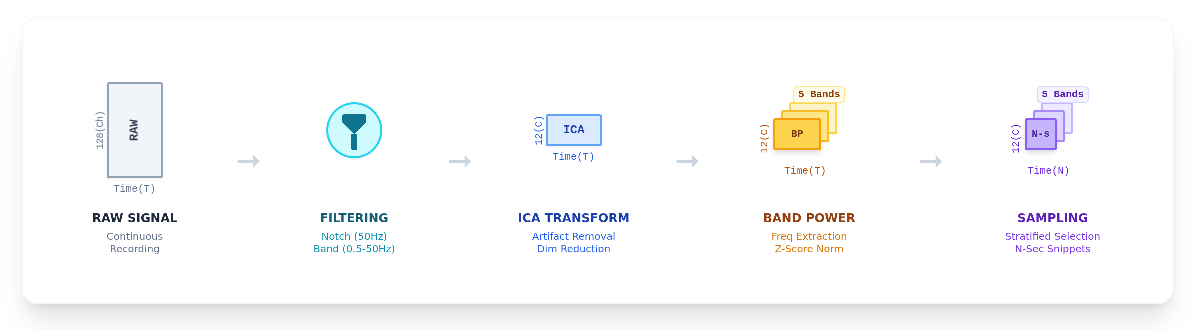
\includegraphics[width=1.1\linewidth]{imgs/preprocessing_pipeline.pdf}}
  \caption{EEG preprocessing pipeline.}
  \label{fig:preprocessing-pipeline}
\end{figure}

\begin{figure}[h]
  \centering
  \begin{minipage}{0.48\textwidth}
    \centering
    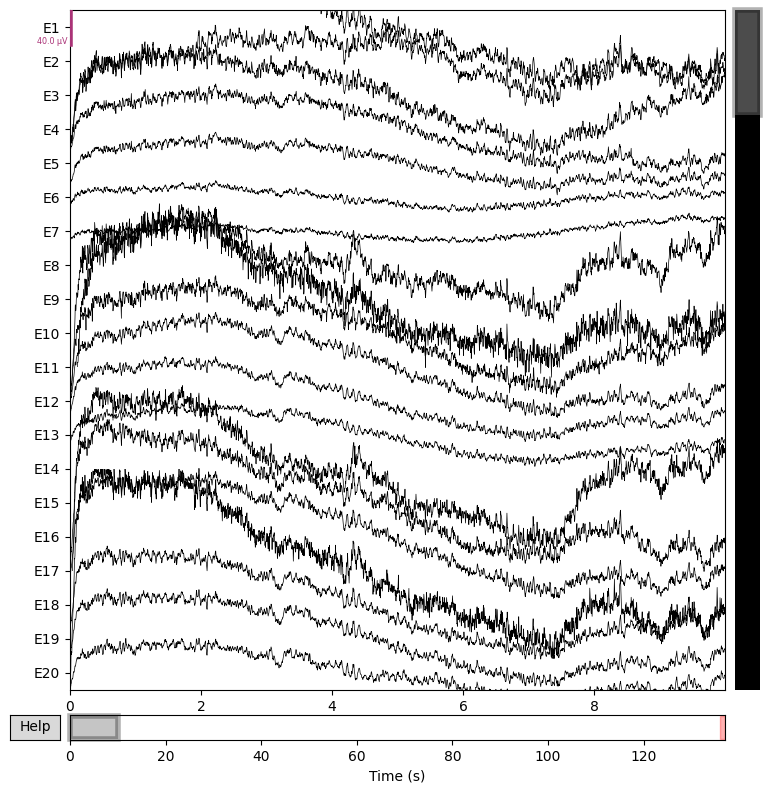
\includegraphics[width=\linewidth]{imgs/eeg_signal_10s_bl_wh.png}
    \caption{EEG signal: 10 second snippet of raw unprocessed EEG signal.}
    \label{fig:eeg-raw}
  \end{minipage}
  \hfill
  \begin{minipage}{0.48\textwidth}
    \centering
    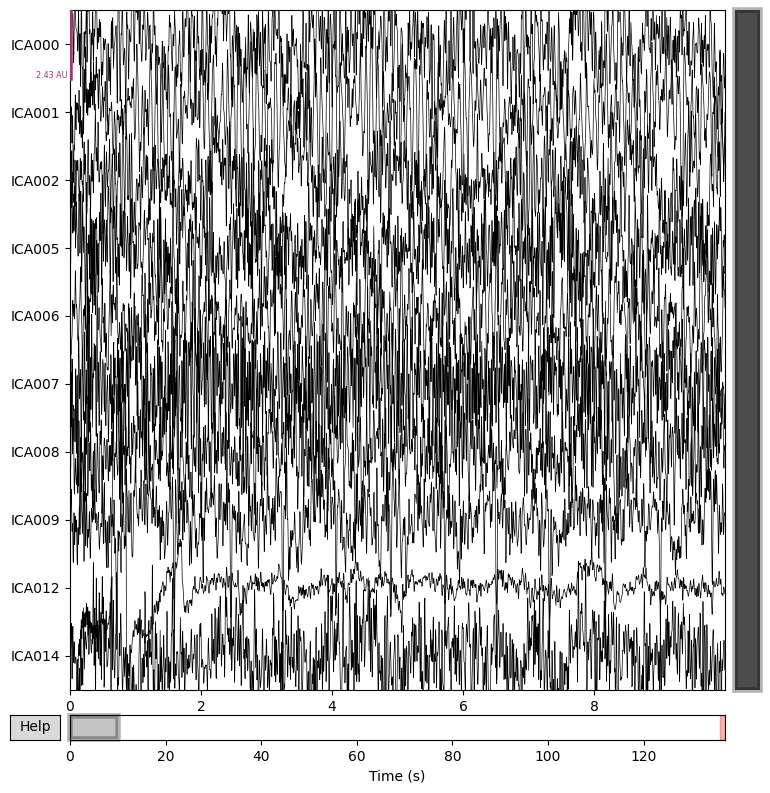
\includegraphics[width=\linewidth]{imgs/ica_signal_10s_bl_wh.png}
    \caption{EEG signal: ICA components.}
    \label{fig:eeg-ica}
  \end{minipage}
\end{figure}

\begin{figure}[h]
  \centering
  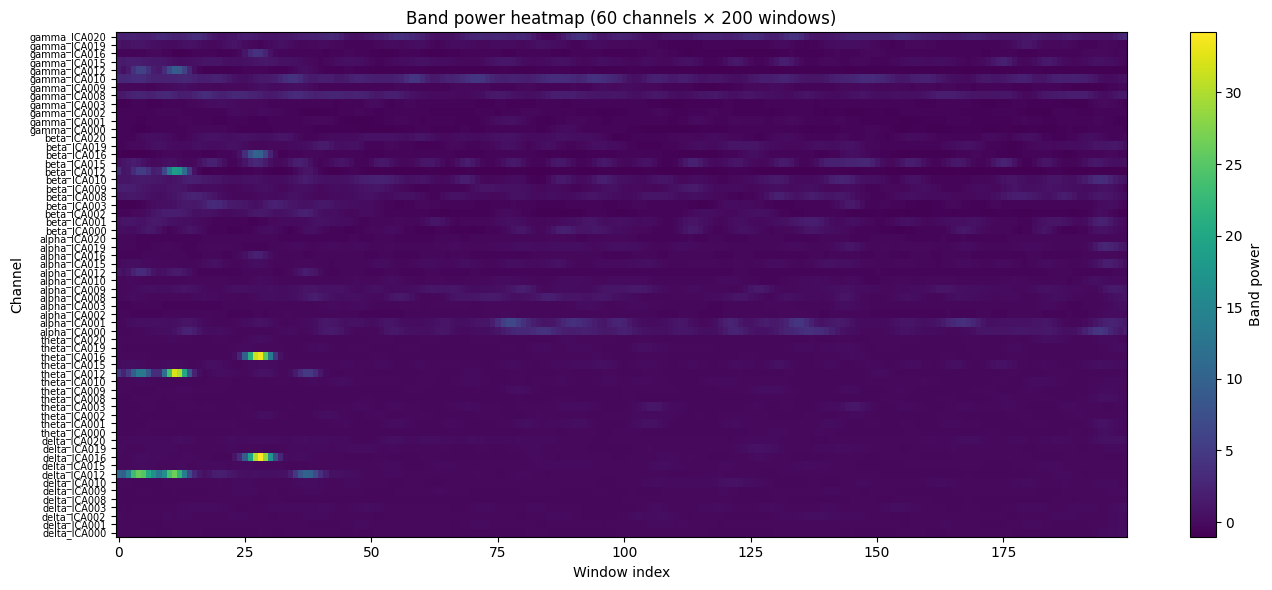
\includegraphics[width=\linewidth]{imgs/ica_band_power_20s.png}
  \caption{Band power of ICA components: 20 second snippet of preprocessed signal.}
  \label{fig:ica-band-power}
\end{figure}

During training, we sample an EEG signal snippet of 3 seconds in length from the full recording.
It was found that varying the length between 3s, 5s, 10s, and 20s impacts classification performance, with longer snippets yielding better accuracy scores\cite{pandey}.
This acts like a data augmentation method.
To avoid the Birthday Problem when randomly sampled segments often strongly overlap over part of the full recording, we 
use stratified sampling method, where first one of \( k \) segments is picked (one after another) and then a random snippet starting within chosen segment is sampled, spreading the distribution more evenly across the whole recording.

\section{Music processing}

\subsection{Spectrogram}

A music spectrogram is a visual representation of the spectrum of frequencies in a sound over time, created by applying a short-time Fourier transform (STFT) to the audio signal.
It is a 2D representation where the x-axis represents time, the y-axis represents frequency, and the intensity or color represents the magnitude of the frequency components at each point in time.
We specifically utilize mel spectrograms, which applies logarithmic scaling to the intensity values to better match human auditory perception.

\subsection{ODF function}
\label{sec:odf}

An odf function is a specific filter on a spectrogram, that responds to the intensity of change in the spectrogram over time.
So, when a spectrogram is relatively constant, the function has values close to 0 and the values are high when there's intense change in the spectrogram, 
where the higher frequency components are counted with stronger weight.

\subsection{Note onset feature extraction}
\label{sec:note-onset}

For the task of detecting note onsets, we use the essentia\cite{essentia} library with its HFC onset detection method to transform the raw wave audio signal into a list of note onset start times.
It first calculates the ODF function and then finds peaks in the function values.

\section{Models}

We use five different model types: KNN, SVM, XGBoost, a Convolutional Neural Network and an LSTM.

\subsection{KNN, SVM, XGBoost}

We employ a KNN model, where a prediction is given by an averaged values of 5 nearest neighbors in euclidean space.
SVM or Support Vector Machines model is a kernel method, where we use the 'Radial Basis Function' kernel.
The XGBoost model is a tree ensamble method, in our case 100 decision trees with a maximum depth of 6 are used together to vote for a prediction.
For a further discussion on the KNN, SVM, and XGBoost models, we refer the reader to Sarker\cite{sarker}\cite{sarker2}.

\subsection{CNN}

We define two related CNN networks: for the classification task and for the music reconstruction task.

\subsubsection{Classification CNN}

The classification network is convolutional neural network with 3 convolutional layers and a fully-connected layer.
It is designed to work with EEG images after preprocessing, which results in 1s snippets of shape \( 60\times 10\).
The model has 35,188 parameters.

% table with layers of cnn 
\begin{table}[h]
\centering
\footnotesize
\begin{tabular}{l|ll}
\hline
\textbf{Layer Type} & \textbf{Filter Size} & \textbf{Input → Output} \\
\hline
Conv2D (freq) & $1 \times 5$ & $[B, 1, 60, 10] \to [B, 16, 60, 10]$ \\
BatchNorm2D & - & $''$ \\
Conv2D (time) & $5 \times 1$ & $[B, 16, 60, 10] \to [B, 32, 60, 10]$ \\
ELU & - & $''$ \\
MaxPool2D & $2 \times 2$ & $[B, 32, 60, 10] \to [B, 32, 30, 5]$ \\
Dropout & - & $''$ \\
\hline
Conv2D (freq) & $1 \times 3$ & $[B, 32, 30, 5] \to [B, 64, 30, 5]$ \\
BatchNorm2D & - & $''$ \\
Conv2D (time) & $3 \times 1$ & $[B, 64, 30, 5] \to [B, 128, 30, 5]$ \\
ELU & - & $''$ \\
MaxPool2D & $2 \times 2$ & $[B, 128, 30, 5] \to [B, 128, 15, 2]$ \\
Dropout & - & $''$ \\
\hline
Conv2D (freq) & $1 \times 3$ & $[B, 128, 15, 2] \to [B, 128, 15, 2]$ \\
BatchNorm2D & - & $''$ \\
Conv2D (time) & $3 \times 1$ & $''$ \\
ELU & - & $''$ \\
MaxPool2D & $2 \times 2$ & $[B, 128, 15, 2] \to [B, 128, 7, 1]$ \\
Dropout & - & $''$ \\
\hline
Flatten & - & $[B, 128, 7, 1] \to [B, 896]$ \\
Linear & - & $[B, 896] \to [B, 4]$ \\
\hline
\end{tabular}
\caption{CNNClassifier model: Classifier model trained on band power data.}
\label{tab:cnn-layers}
\end{table}

\subsubsection{Reconstruction CNN}

The reconstruction network uses a U-Net style architecture with a 3-layer contracting encoder, a middle bottleneck fully connected layer, and a 3-layer expanding decoder.
The encoder has the same architecture as the classifier model, and the decoder is correspondingly a 3-layer upsampling convolutional network.
There are skip connections between matching layers of the encoder and decoder.
Because the input has a different dimensionality than the output and consequently, the outputs of the encoder and decoder layers differ in shape, the skip connections also apply interpolation to match the dimensions.
The model has 143,280 parameters.

We also define a simplified version of the reconstruction network, which aims to reconstruct spectrograms which are constant in the time dimension.
This significantly reduces complexity and allows to remove decoder part of the model.
Both full (CNNReconstruction) and simplified (CNNReconstructionMel) architectures are visible in Figure~\ref{fig:cnn-diagrams}.

\begin{figure}[h]
  \centering
  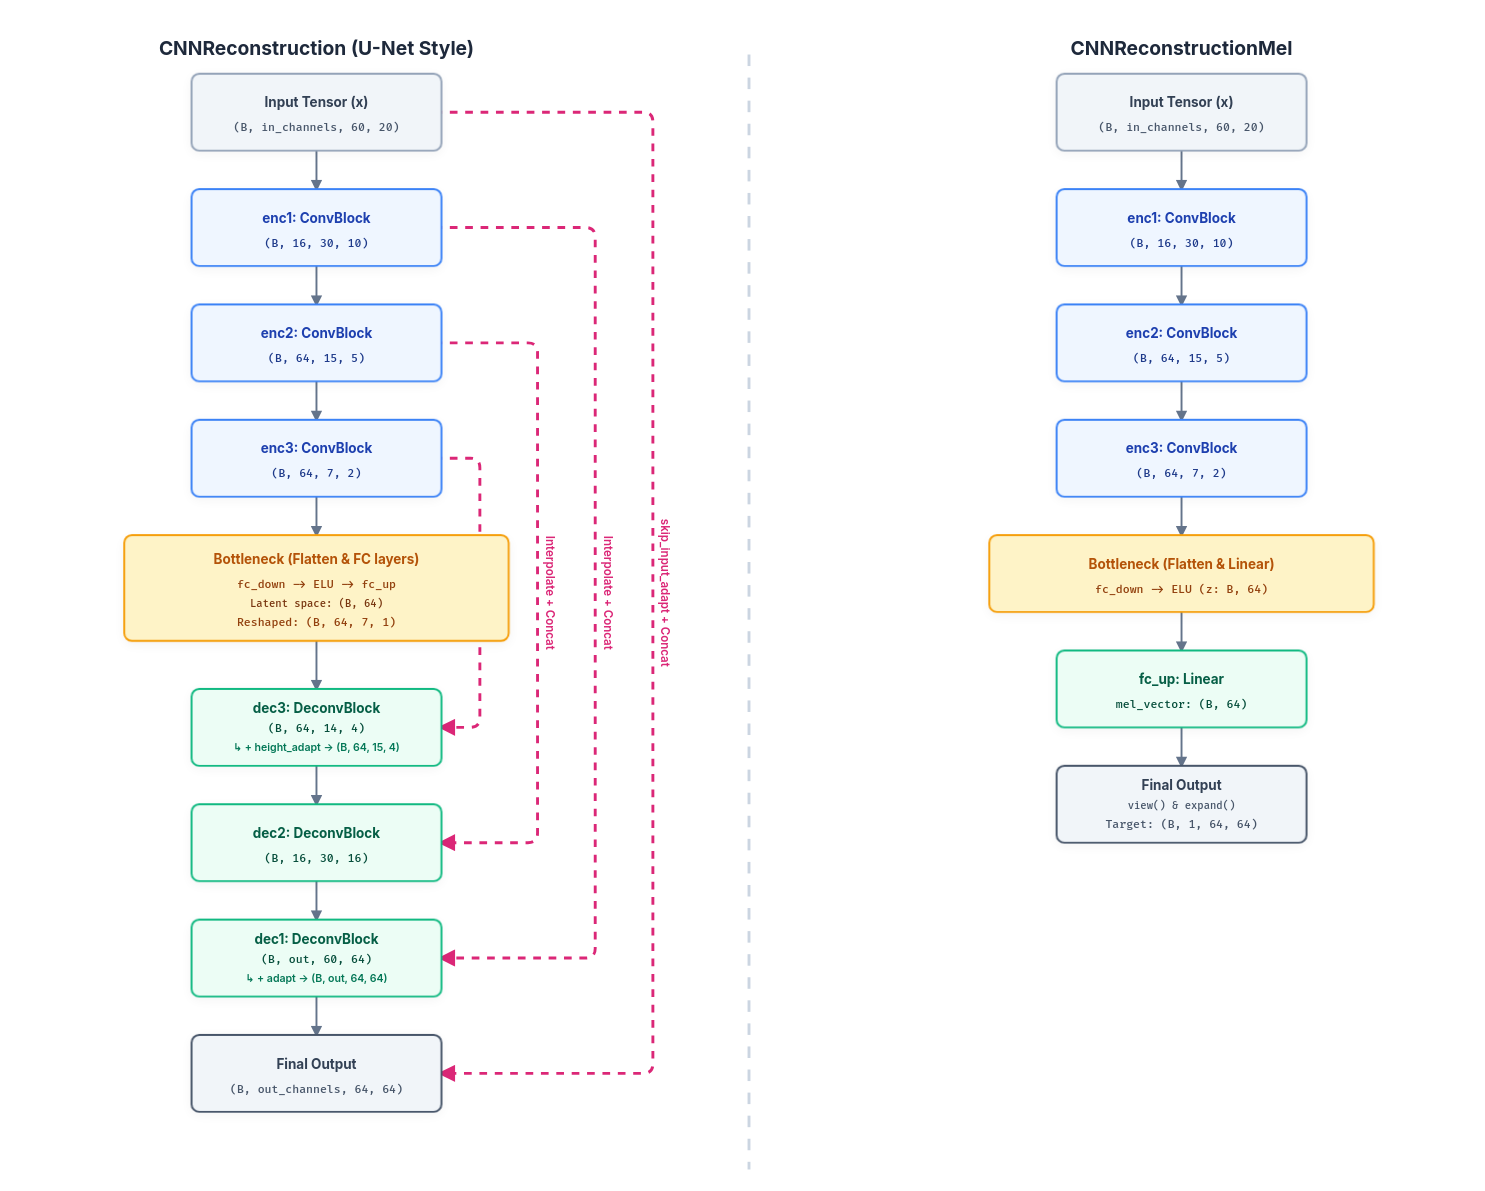
\includegraphics[width=\textwidth]{imgs/cnn_diagrams.png}
  \caption{Architecture diagrams of the full reconstruction CNN (U-Net style with encoder, bottleneck, and decoder with skip connections) and the simplified time-constant variant (encoder followed by a single fully connected layer producing a $64\times1$ output broadcasted to $64\times64$).}
  \label{fig:cnn-diagrams}
\end{figure}

\begin{table}[h]
\centering
\footnotesize
\begin{tabular}{l|ll}
\hline
\textbf{Layer Type} & \textbf{Filter Size} & \textbf{Input → Output} \\
\hline
\multicolumn{3}{c}{\textit{Encoder}} \\
\hline
Conv2D (freq) & $1 \times 5$ & $[B, 1, 60, 10] \to [B, 16, 60, 10]$ \\
BatchNorm2D & - & $''$ \\
Conv2D (time) & $5 \times 1$ & $[B, 16, 60, 10] \to [B, 32, 60, 10]$ \\
ELU & - & $''$ \\
MaxPool2D & $2 \times 2$ & $[B, 32, 60, 10] \to [B, 32, 30, 5]$ \\
Dropout & - & $''$ \\
\hline
Conv2D (freq) & $1 \times 3$ & $[B, 32, 30, 5] \to [B, 64, 30, 5]$ \\
BatchNorm2D & - & $''$ \\
Conv2D (time) & $3 \times 1$ & $[B, 64, 30, 5] \to [B, 128, 30, 5]$ \\
ELU & - & $''$ \\
MaxPool2D & $2 \times 2$ & $[B, 128, 30, 5] \to [B, 128, 15, 2]$ \\
Dropout & - & $''$ \\
\hline
Conv2D (freq) & $1 \times 3$ & $[B, 128, 15, 2] \to [B, 128, 15, 2]$ \\
BatchNorm2D & - & $''$ \\
Conv2D (time) & $3 \times 1$ & $''$ \\
ELU & - & $''$ \\
MaxPool2D & $2 \times 2$ & $[B, 128, 15, 2] \to [B, 128, 7, 1]$ \\
Dropout & - & $''$ \\
\hline
\multicolumn{3}{c}{\textit{Bottleneck}} \\
\hline
Flatten & - & $[B, 128, 7, 1] \to [B, 896]$ \\
Linear + ELU & - & $[B, 896] \to [B, 128]$ \\
Unsqueeze & - & $[B, 128] \to [B, 128, 1, 1]$ \\
ConvTranspose2D & $7 \times 1$ & $[B, 128, 1, 1] \to [B, 128, 7, 1]$ \\
\hline
\multicolumn{3}{c}{\textit{Decoder}} \\
\hline
Concat (skip enc3) & - & $[B, 128, 7, 1] + [B, 128, 7, 1] \to [B, 256, 7, 1]$ \\
Upsample & $2 \times 4$ & $[B, 256, 7, 1] \to [B, 256, 14, 4]$ \\
Conv2D (time) & $3 \times 1$ & $[B, 256, 14, 4] \to [B, 128, 14, 4]$ \\
BatchNorm2D & - & $''$ \\
Conv2D (freq) & $1 \times 3$ & $''$ \\
ELU & - & $''$ \\
Dropout & - & $''$ \\
AdaptiveAvgPool2D & - & $[B, 128, 14, 4] \to [B, 128, 15, 4]$ \\
\hline
Concat (skip enc2) & - & $[B, 128, 15, 4] + [B, 128, 15, 4] \to [B, 256, 15, 4]$ \\
Upsample & $2 \times 4$ & $[B, 256, 15, 4] \to [B, 256, 30, 16]$ \\
Conv2D (time) & $3 \times 1$ & $[B, 256, 30, 16] \to [B, 64, 30, 16]$ \\
BatchNorm2D & - & $''$ \\
Conv2D (freq) & $1 \times 3$ & $[B, 64, 30, 16] \to [B, 32, 30, 16]$ \\
ELU & - & $''$ \\
Dropout & - & $''$ \\
\hline
Concat (skip enc1) & - & $[B, 32, 30, 16] + [B, 32, 30, 16] \to [B, 64, 30, 16]$ \\
Upsample & $2 \times 4$ & $[B, 64, 30, 16] \to [B, 64, 60, 64]$ \\
Conv2D (time) & $5 \times 1$ & $[B, 64, 60, 64] \to [B, 16, 60, 64]$ \\
BatchNorm2D & - & $''$ \\
Conv2D (freq) & $1 \times 5$ & $[B, 16, 60, 64] \to [B, 1, 60, 64]$ \\
ELU & - & $''$ \\
Dropout & - & $''$ \\
\hline
\multicolumn{3}{c}{\textit{Final Adaptation}} \\
\hline
Conv2D + ELU & $3 \times 3$ & $[B, 1, 60, 64] \to [B, 1, 60, 64]$ \\
AdaptiveAvgPool2D & - & $[B, 1, 60, 64] \to [B, 1, 64, 64]$ \\
Concat (skip input) & - & $[B, 1, 64, 64] + [B, 1, 64, 64] \to [B, 2, 64, 64]$ \\
Conv2D & $1 \times 1$ & $[B, 2, 64, 64] \to [B, 1, 64, 64]$ \\
\hline
\end{tabular}
\caption{CNNReconstruction model: U-Net style network for music spectrogram reconstruction.}
\label{tab:cnn-reconstruction-layers}
\end{table}


\subsection{DTW}

DTW is an algorithm that finds an optimal alignment between two sequences.

We employ a generalized version called approximate-subsequence-DTW, which can be defined by:
\begin{enumerate}
  \item Given two sequences $A$ and $B$, it finds a match between an infix of $A$ and infix of $B$.
  \item The summed distances between the matched points are within the cost allowance.
  \item The matched infix is of maximal length.
\end{enumerate}

This means that the algorithm pairs points from one sequence, or just an infix of it, with points from the other sequence.
As many points are matched as is possible within the cost constraint, which specifies what is the sum of differences between the matched points.
The algorithm is a variant of the standard DTW dynamic programming algorithm.

\subsection{LSTM}

LSTM, or more specifically Bi-LSTM (an LSTM with bidirectional information flow), is a recurrent neural network operating on raw EEG timeseries.
We use variants operating on 12 or 129 EEG channels, with 2 hidden layers and 256 hidden units.
The output of the network is a scalar.

% \section{Neurals Networks}

% \section{XGBoost}

% \section{SVM}

% https://pubmed.ncbi.nlm.nih.gov/40039043/

% \section{KNN}



\chapter{Datasets}

We run our experiments on two datasets: MUSIN-G\cite{musing} and what we call BCMI-training\cite{bcmi}.
Both contain joint EEG and music recordings, but while MUSIN-G contains natural music, BCMI-training contains computer-generated music.
We choose the two datasets to test our hypothesis both on generated but uniform and natural music.

\section{MUSIN-G}

It is a dataset of joint music and EEG recordings of 20 non-musician subjects, aged 22-28 years\cite{musing}.
Data was acquires using high-density Hydrocel Geodesic Sensor Net.
Each subject was presented with 12 songs of various genres, ranging from Indian Folk to Electronic Dance.

\begin{table}[h]
\centering
\begin{tabular}{|l|l|l|c|}
\hline
Song Name & Artist & Genre & Length (s) \\
\hline
Trip to the Lonely Planet & Mark Alow & Deep House & 125 \\
Sail & AWOLNATION & Electric Pop & 114 \\
Concept 15 & Kodomo & Electronic & 132 \\
Aurore & Claire David & New Age & 111 \\
Proof & Idiotape & Electronic & 124 \\
Glider & Tycho & Slow Electronic & 100 \\
Raag Bihag & Pandit Hariprasad Chaurasia & Hindustani Classical & 116 \\
Albela Sajan & Shankar Mahadevan & Indian Semi-Classical & 121 \\
Mor Bani Thanghat Kare & Aditi Paul & Indian Folk & 126 \\
Fallin & Dr. SaxLove & Soft Jazz & 129 \\
Master of Running & Rickeyabo & Goth Rock & 113 \\
JB & Nobody.one & Progressive Instrumental & 117 \\
\hline
\end{tabular}
\caption{MUSIN-G dataset songs}
\label{tab:musing-songs}
\end{table}



\section{BCMI-training}

BCMI-training is a dataset of joint music and EEG recordings of 10 participants aged 19-30.
It is part of a series of datasets collected during studies investigating human reactions to affective musical stimuli and whether reported emotionality can be influenced by music\cite{nicolaou}.
The music played in this study is fully computer-generated, and no track repeats across the dataset.
The musical snippets are tagged with emotionality labels (9 possibilities on valence/arousal grid) which are inputs to the music generation algorithm.
In the study, subjects listened to a musical snippet of about 20 seconds in length and immediately afterward to another snippet of different emotionality.
For our purposes, we split such trials into two separate recordings, one for each snippet.

\section{Dataset processing}

The raw datasets are preprocessed for the use in our experiments.
To efficiently construct various variants of the datasets, including different preprocessing methods, we created a library for dataset handling and processing.
The library itself uses libraries like "librosa" and "essentia" for audio processing and "mne" for EEG processing.
The library allows for loading of the two datasets to a common format, lazy evaluation of preprocessing steps, defines a standard on disk storage format and simplifies dataset operations like filtering. 
It also allows to combine datasets, but we didn't end up using this feature.
We show below how a dataset is loaded for a study using our library.

We unify the various analyzed datasets under the `EEGMusicDataset` class, which provides a common interface to access the data and metadata of the recordings.
Then, various preprocessing functions are applied to the data; their evaluation is lazy.
Lastly, the `StratifiedSamplingDataset` wrapper is applied, which samples the data in a stratified way, as described in the methods chapter.

\begin{verbatim}
ds = EEGMusicDataset.load_ondisk(Path("..."))

ds = MappedDataset(ds, lambda x: 
  ica_band_power_trial(
    rereference_trial(
      filter_trial(
        notch_filter_trial(x, 50.0), l_freq=0.5, h_freq=50.0
      )
    ),
    n_components=12,
    bands = [(0.5, 4), (4, 8), (8, 13), (13, 30), (30, 45)],
    window_sec= 2.0,
    hop_sec = 0.1,
  )
)

ds = StratifiedSamplingDataset(ds, n_strata=10, trial_length_secs=Fraction(3, 1))

\end{verbatim}

% musing


% grupa bcmi:
%  - opis eksperymentu
%  - używamy treningowego, choć można połączyć



\chapter{Related work}

\section{Music classification}

Classification of listened music based on EEG signal has been tackled in various forms by several researchers.

As early as 2011, a linear logistic-regression classifier was successfully used to classify ERP (event-related potential) segments of EEG signals into listened-to songs\cite{rebecca}.
The focus on ERPs means that every trial, which is slightly over 3 seconds long, acts as its own snippet for classification. Therefore, the EEG snippets are aligned in time --- all starting when the music began playing in the experimental scenario.

In a similar paradigm, Sterni et al.\cite{sterni} classify listened-to music using first a dimensionality reduction technique to learn signal components, and then a CNN with a single convolutional layer.
They also succeed in classifying trials based on the meter of a song (3/4 versus 4/4).

Two studies, linked by the collected dataset later published as MUSIN-G, tackle the problem of classifying listened-to music based on the EEG signal in a paradigm similar to ours, 
where a snippet for classification is randomly sampled from the entire recording.
A study by Lawhatre uses a multilevel wavelet method, which finds frequency components at various time scales, to extract lower-level features and then tests various models such as KNN, decision trees, SVM, and CNNs\cite{lawhatre}.
The study establishes the usefulness of the dataset.

The second study applies a 3-layer CNN to either the time-domain EEG signal or the frequency-domain spectrogram of the EEG\cite{guess}.
It does not perform better than a random classifier in the time-domain case.
However, in the frequency-domain case, the best CNN model with ~1.6M parameters achieved over 80\% accuracy.
In the cross-participant setting, however, the model failed to generalize.

The existence of a signal related to music in the EEG signal poses a question: what about imagining music?
In a 2021 paper, researchers attempted to classify EEG by first decoding EEG from music\cite{silence}.
The musical input is transformed into a binary vector that encodes note onsets, together with an auxiliary vector that encodes expected note surprise,
as calculated by a mathematical model of musical expectation in sheet music.
For every music track, the predicted matching EEG is compared against the real EEG signal, and the one with the strongest match is chosen.
Separate models were trained for the listened and imagined music, but it was also shown that they relate to each other, with the listened version being a lagged version of the imagined one.

\section{Representation learning}

Stober et al. approach a more general problem of learning representations of the EEG signal with a convolutional autoencoder\cite{stober}.
To combat the small and noisy dataset, the model is trained on a given trial to reconstruct a possibly different trial, but of the same subject and stimulus.
They are able to train CNN and SVC classifiers to predict the song ID from the hidden representation of the autoencoder.

This raises the question of whether a common representation space could be found for both music and the EEG signal, or if the two can be related to each other.
Researchers attempted to answer the second question by comparing the distance matrices within the sets of extracted audio features and extracted EEG features\cite{foster}.
The study reports mixed results.

% \cite{rebecca} - 2011, quadratically regularized linear logistic-regression classifier, 3s event-aligned EEG segments

% \cite{sterni} - 2016, time signature (3/4 versus 4/4), lyrics (music with lyrics versus
% music without), tempo (slow versus fast), and instrumentation. classification 28\% acc of real but not imagined

% \cite{lawhatre} - collects dataset, extracts lowdim features (multilevel wavelet, ours is like one chosen level) and tests with various models, trial-split
% \cite{guess} - created dataset, trial split, cnn time and frequency domain experiments

% \cite{stober} - deep feature learning using CAE

% \cite{foster} - performs comparison of EEG extracted features as dataset and music features dataset (with distance matrices) AND by using linear regression
% also does song id prediction with logistic regression and 28\% accuracy

% \cite{silence} - found similarity between brains neural responses to note onset and surprise between listened and imagined



\section{Music reconstruction}

Works of the last few years tackled the harder problem of reconstructing listened music from the EEG signal.

The simplest approach seems to be directly training a function that maps the EEG signal to music.
A 2022 study attempts this with a 5-layer CNN model\cite{kello}.
The network is fed 1s snippets, randomly sampled from the full recording and assigned to the training set with a 75\% probability, and outputs audio in the form of a mel spectrogram. 
The accuracy of the model is assessed by training a classifier to predict the song ID from the reconstructed music, achieving over 80\% accuracy.
The model outputs were also evaluated by human listeners, who were able to successfully determine which of two presented audio clips corresponded to a third target sound.

The diffusion approach to music generation was tested in a 2025 study\cite{postolache}.
The music is generated via a diffusion process in the latent space, where initial noise is iteratively refined with a denoising network.
The denoised latent variable is then fed into a decoder that converts it into an audio spectrogram.
The denoising model is a pretrained AudioLDM2 model, trained on a general music generation task.
The researchers trained a ControlNet\cite{controlnet} adapter to condition the denoising network on the EEG signal.
The results are quantified using metrics applicable to generation tasks, such as FAD or the Pearson correlation coefficient.

There are also attempts at combining EEG with fMRI data\cite{daly}.
The fMRI signal allows for the localization of sources of neural activity.
EEG processing can use this information to translate the EEG signal into an equivalent one, as if it were recorded with electrodes at the sites of activity.
This processed EEG constitutes the input to a biLSTM model. The model is able to reconstruct the music in waveform. A separate model is trained for every study subject.
The output quality is evaluated by calculating the similarity between the reconstructed audio and all the listened-to songs, and then ranking them based on similarity.
Importantly, even without the fMRI-influenced processing step, the results are positive, albeit worse.

Only fMRI was used in a 2023 study\cite{denk}, which relies on the MuLan music encoder and the MusicLM music decoder.
Here, the chosen voxels of the fMRI signal are an input to a linear regression model that is trained to predict the embeddings of the music as given by the MuLan encoder model.
Then, the MusicLM model generates audio from the predicted embeddings.

Described attempts show that the task while hard is not impossible.

% Daly\cite{daly} succesfully tackles the harder problem of reconstructing

% https://gemini.google.com/app/d5570707986ff8b1

% https://gemini.google.com/app/b6c26a36626bc5ee

% Full decoding.


\chapter{Experiments}

We attempt to decode progressively harder features of the music signal from the EEG recordings.
We utilize the preprocessing pipeline described in the previous section.
For the Bi-LSTM model, we skip the final band power extraction step and feed the filtered EEG signal directly to the network.

\section{Song name prediction}

We start with the task of predicting the song name of a listened-to song based on the EEG signal.
We split the MUSIN-G dataset into recordings of 12 subjects for training and the remaining 8 subjects for testing (for CNN, half of the test set serves as the validation set).
We then train a model to predict the song name from the EEG signal.
We achieve the below results for each variant of the tested model.
For the CNN model we provide the best result out of the few tested variants, described below.

\begin{table}[h]
  \centering
  \begin{tabular}{|l|c|}
    \hline
    \textbf{Model} & \textbf{Accuracy} \\
    \hline
    Random  &  0.0833  \\
    KNN     & 0.1374 \\
    SVM     & 0.1229 \\
    XGBoost & 0.1668 \\
    CNN (best)      & \textbf{0.1802} \\
    \hline
  \end{tabular}
  \caption{Song name prediction accuracy: subject-wise split.}
  \label{tab:song-prediction}
\end{table}


Our results are comparable to the study by Pandey et al.\cite{pandey}, in which researchers achieved 12.5\% mean subject accuracy (a random classifier gives \(  \frac{1}{12} = 0.08(3) \)).

We also tested how the number of parameters influences the model's performance. We kept the architecture and varied number of convolution channels. The results are shown below.

\begin{figure}[h]
  \centering
  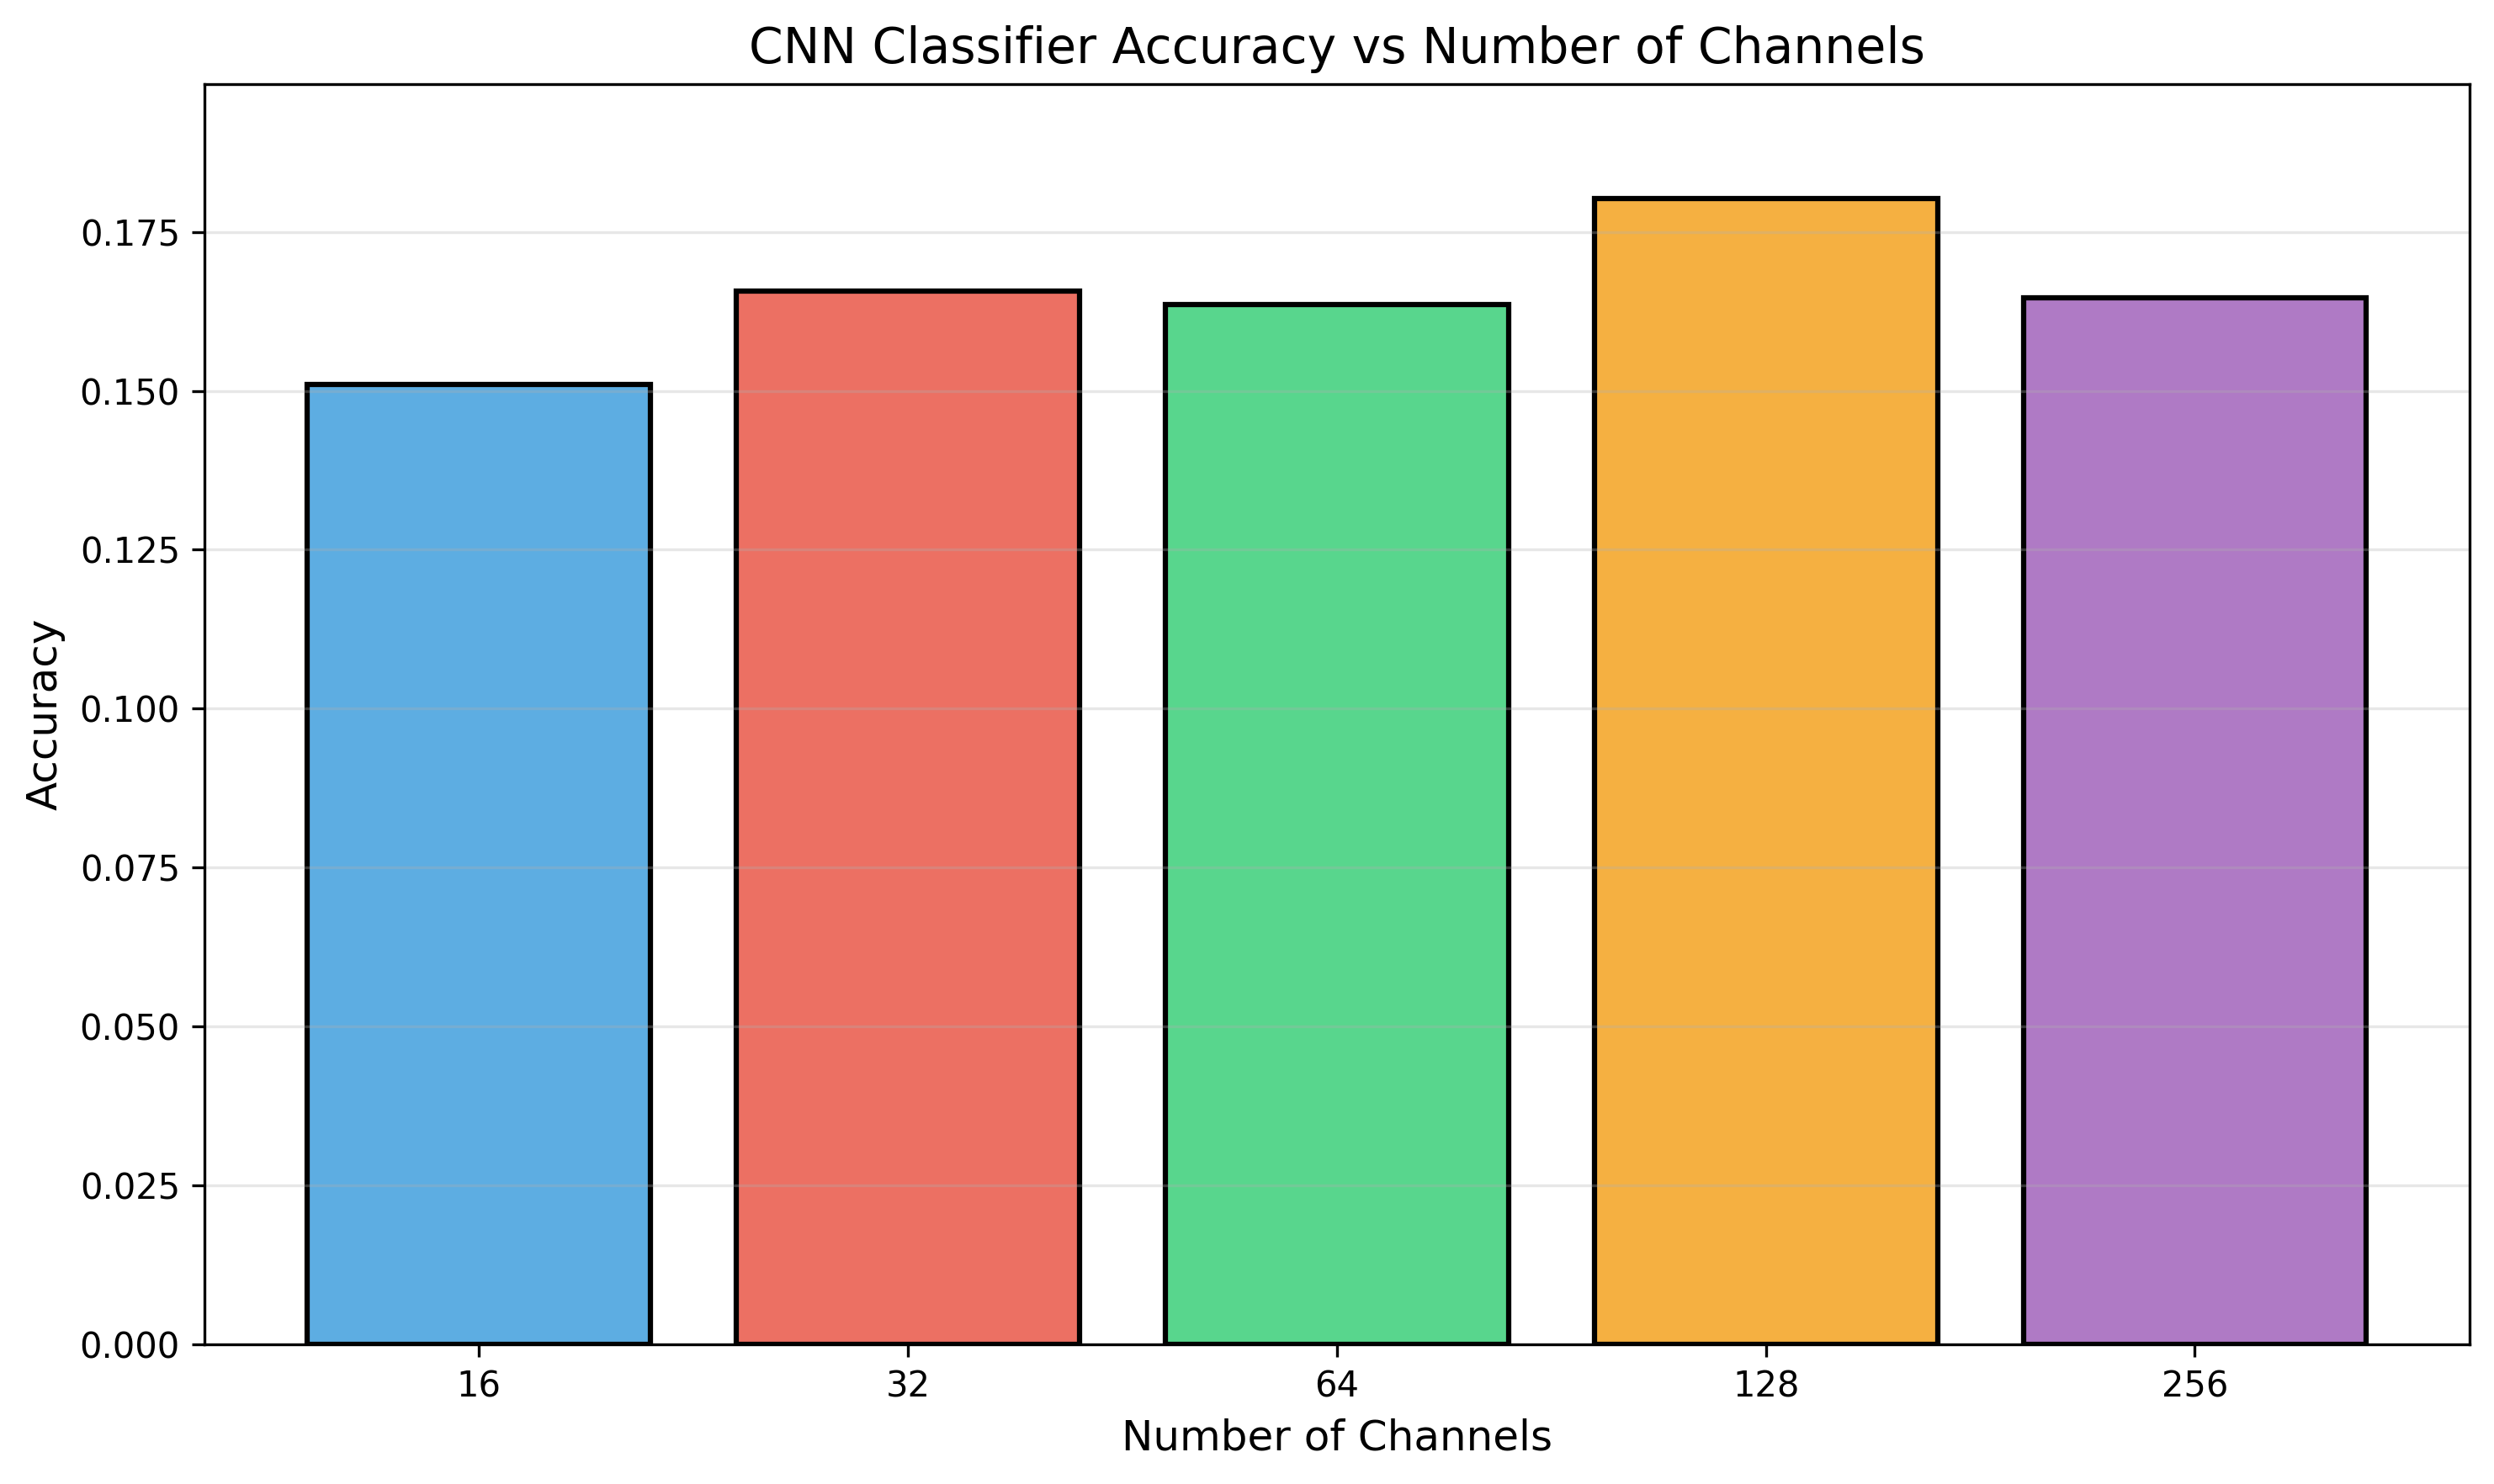
\includegraphics[width=0.7\linewidth]{imgs/cnn_channels_accuracy.png}
  \caption{CNN accuracy as a function of the number of convolution channels.}
  \label{fig:cnn-channels-accuracy}
\end{figure}


In the above study, researchers also tested scores achieved in a different testing paradigm. They split the MUSIN-G dataset into training and testing 
by taking the initial \( n \) seconds of each recording as training data and the remaining seconds as testing data. The study compares results that can be achieved for a few chosen \( n \) parameters (\(3, 5, 10, 20\)), achieving higher accuracy for larger training partitions.
The results in this variant of the experiment are much higher (\( 84\% \)) than in the previous variant.
We are able to reproduce these results, and for \( n=20 \) we achieve accuracies as shown in the table:

\begin{table}[h]
  \centering
  \begin{tabular}{|l|c|}
    \hline
    \textbf{Model} & \textbf{Accuracy} \\
    \hline
    XGBoost & \textbf{0.85} \\
    SVM     & 0.57 \\
    KNN     & 0.64 \\
    NN      & 0.72 \\
    \hline
  \end{tabular}
  \caption{Song id prediction accuracy in the MUSIN-G dataset: temporal split.}
  \label{tab:song-id-temporal-split}
\end{table}

While the best model in the trial-wise split variant achieves 0.85\% accuracy, the best model in subject-wise split variant achieves only 0.18\%.
This means that the model fails to learn neural patterns that generalize across subjects.
This poor generalization suggests that the model in this trial-wise variant does not pick up on neural correlates of the music but rather on some trial-specific aspects of the EEG recording.
We test the hypothesis with two experiments. 

First, we run a similar experiment on the BCMI-training dataset. The dataset contains from 144 up to 432 trials recorded for a single subject.
The recordings share the ``emotionality'' of the listened-to music, but no listened-to song repeats across the dataset as the songs are computer-generated for each trial.
We find that, similarly to the study, classifiers are able to predict the trial ID from the EEG signal with high accuracy. 
The results are shown in the below table.

\begin{table}[h]
  \centering
  \begin{tabular}{|l|c|}
    \hline
    \textbf{Model} & \textbf{Accuracy} \\
    \hline
    XGBoost & 0.78 \\
    SVM     & \textbf{0.91} \\
    KNN     & 0.88 \\
    CNN      & ---    \\
    \hline
  \end{tabular}
  \caption{Song id prediction experiment in the BCMI-training dataset.}
  % \caption{Song id prediction experiment in the single subject variant in the BCMI-training dataset.}
  \label{tab:song-id-single-subject}
\end{table}

\subsection{DTW-based trial id prediction}

Secondly, guided by the intuition that the classifiers notice directly repeatable patterns in the EEG signal between training and test sets and are not forced to generalize beyond that, we propose the following experiment.
We attempt to predict the trial ID using the DTW algorithm.

DTW in its most basic form is a method of measuring the distance between two time series by finding an optimal alignment between them.
Such an alignment is a match between points of one time series and points of the other time series that minimizes the sum of distances between matched points, 
starts and ends at the two matched ends of the two time series, and is monotonic in between. 

We employ a version of the algorithm called approximate-subsequence-DTW, described in the methods section.
The algorithm allows for calculation of alignment cost between some infixes of the two sequences.
We use it to compare a "similarity" of one sequence to another.
Running it on two EEG sequences, we find what is the longest fragment that approximately repeats across the two signals.
Matching a test trial with every trial from a training set and comparing the lengths of the matches, we can find the most similar trial and use it to assign a prediction.

For a single subject of the BCMI-training dataset, we predict the trial ID of a test trial by finding, across all training trials,
the one that scores the highest when calculating the approximate-subsequence-DTW distance between the test trial and the training trial.
We fit the cost allowance hyperparameter on the validation set and then test the accuracy of the method on the test set. 
The cost parameter specifies how much cummulative difference between the matched points of the two sequence we allow.
With this simple method we achieve 50.83\% test accuracy.
% Accuracy: 61/120 = 50.83%
The experiment is meant to showcase that such direct pattern matching is possible and therefore---it is possible for the model to learn it and rely on it greatly, with little generalization capability.

\section{Emotion prediction}

The BCMI-training dataset is made of computer-generated snippets of music. These musical snippets are tagged with emotionality labels, one of 9 possibilities arranged on Valence and Arousal axes.
To compare the difficulty of this task with previous tasks, we can think of emotionality labels as abstraction classes that join multiple individual trials together.
Therefore, it is easier to predict an emotion label than an identifier, as this requires less precision, but during training, the 
reward per training step is less valuable and gives less information.
The balance does not seem to be in favor of this task, as we are unable to achieve good results, even though we do in the prediction task.

\begin{table}[h]
\centering
\begin{tabular}{l c}
\hline
Method  & Accuracy \\
\hline
XGBoost & 0.1089 \\
SVM     & 0.1123 \\
KNN     & 0.1117 \\
CNN     & \textbf{0.1130} \\
\hline
\end{tabular}
\caption{Emotion prediction accuracy}
\label{tab:emotion-prediction}
\end{table}

\section{Music ``density'' prediction}

Looking for musical features visible through the EEG recording, we define a ``density'' of a music snippet and, by extension, the paired EEG snippet.
First, we mark note onsets in the music recordings. 
We do that by looking at the music's mel spectrograms and marking the time points at which the spectrogram's energy increases significantly, weighting the changes in the high frequencies more (High-Frequency-Content method).
The HFC method was visually compared to other methods and chosen as seemingly best.

\begin{figure}[h]
  \centering
  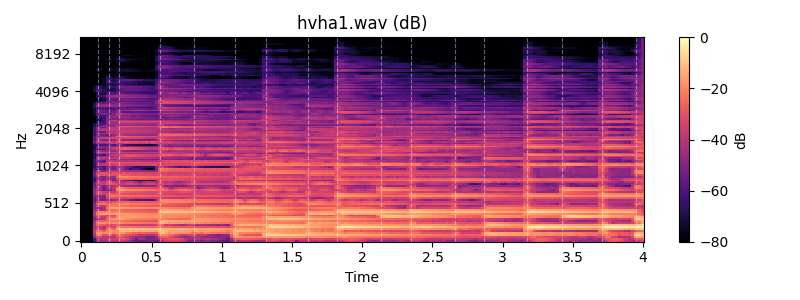
\includegraphics[width=\linewidth]{imgs/mel_onset_hvha1.wav.png}
  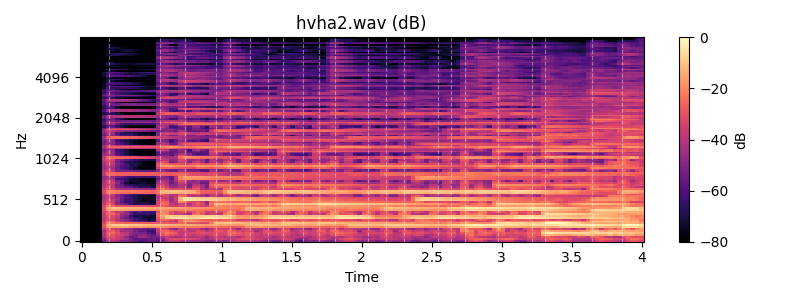
\includegraphics[width=\linewidth]{imgs/mel_onset_hvha2.wav.png}
  \caption{Spectrograms of two 4s music snippets with marked note onsets.}
  \label{fig:mel-onsets}
\end{figure}

Now, for a chosen length of a time window, we get a certain distribution of the number of note onsets within windows of this length.
Calculating the median number, we can split the snippets into two classes: the ``sparse'' class with a number of onsets below the median, and the ``dense'' class with a number of onsets above the median.
We calculate the median only on the training set and define a classification task of predicting the class of a snippet based on the paired EEG snippet.
We hope that success in this task may be a stronger indicator that some musical features are present and can be decoded from the EEG signal.

Results are shown in the table below.

\begin{table}[h]
  \centering
  \begin{tabular}{|l|c|}
    \hline
    \textbf{Model} & \textbf{Accuracy} \\
    \hline
    XGBoost & \textbf{0.5407} \\
    SVM     & 0.5093 \\
    KNN     & 0.5264 \\
    CNN     & 0.5206 \\
    \hline
  \end{tabular}
  \caption{Music density prediction accuracy.}
  \label{tab:density-prediction}
\end{table}

\section{Music reconstruction}

We attempt to reconstruct listened-to music from the EEG signal for the MUSIN-G dataset.
We treat this task as an extension of the song ID prediction task: if a model can learn to predict a song, can it learn to predict the specific fragment of a song and generate its mel spectrogram?
Our architecture of the $CNN_{reconstruction}$ model used for this task reflects this idea. 
It can be seen as an encoder and decoder model, with skip connections, where the encoder is similar to the $CNN_{classification}$ model.

Reflecting the results in the song identification tasks, we observe that the model is able to reconstruct music to some extent in the variant where 
single-subject recordings are split into training and test partitions by assigning the initial 20s of each recording to training.
The reconstructions are accurate enough to allow for meaningful classification (see figures below). 

In the cross-subject variant, where we investigate the ability for cross-subject generalization and a different portion of subjects is used for training and testing, 
we don't achieve any meaningful results in the reconstruction task. 
This matches the established accuracies in the song ID prediction task for this variant, which were much lower and were all between 12\% and 18\%, compared to the 57\% to 85\% range.


\begin{figure}[h]
  \centering
  \textbf{Accuracy scores in the temporal-split}
  \vspace{0.3cm}
  
  \begin{minipage}[t]{0.48\textwidth}
    \centering
    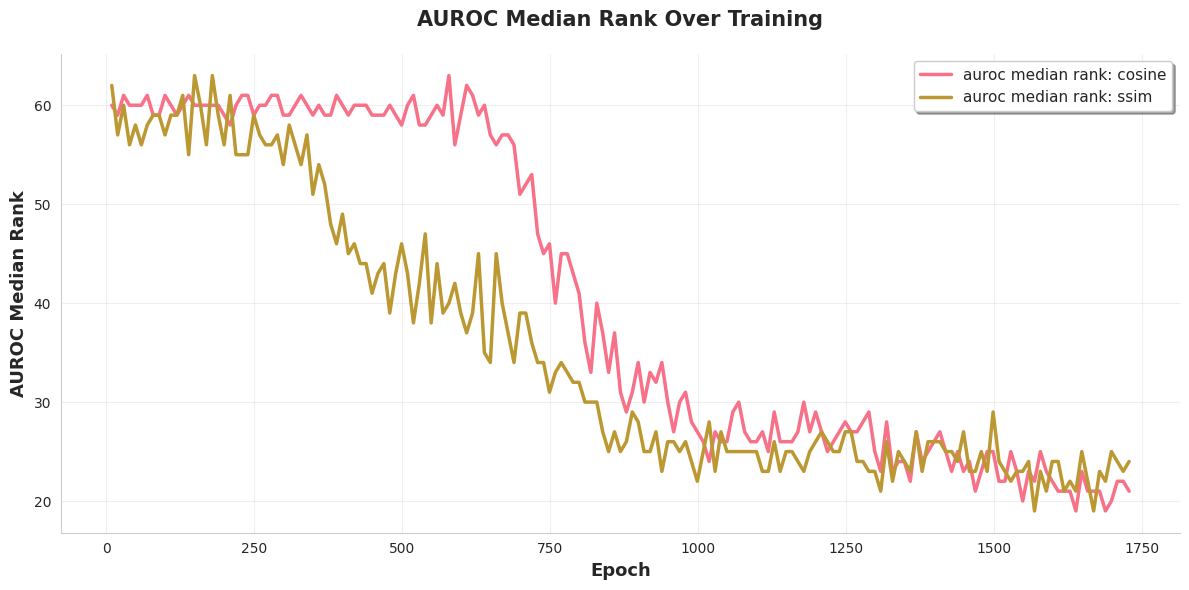
\includegraphics[width=\textwidth]{imgs/auroc_median_rank_plot.png}
    \caption{For a generated mel spectrogram, we calculate similarities with all 120 real spectrograms from the current batch. We then sort the spectrograms based on the similarity scores and find out what the rank of the true spectrogram is to assess the quality of our predicted one. The plot shows the median rank for two used similarity measures: cosine similarity and structural similarity.}
    \label{fig:auroc-median-rank}
  \end{minipage}
  \hfill
  \begin{minipage}[t]{0.48\textwidth}
    \centering
    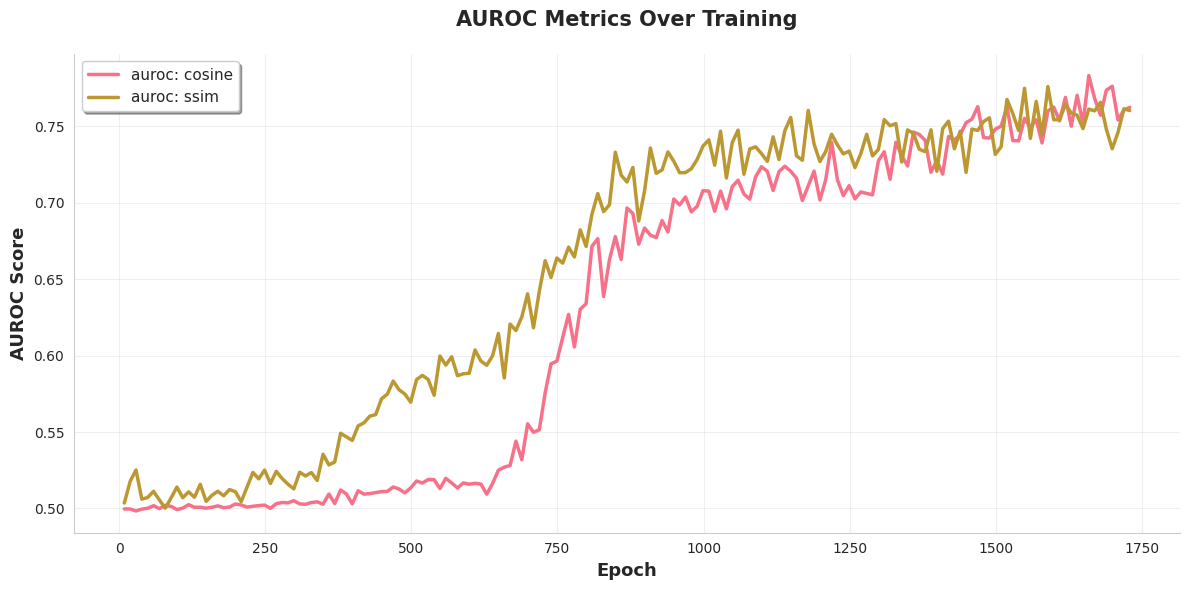
\includegraphics[width=\textwidth]{imgs/auroc_score_plot.png}
    \caption{AUROC score counts the ratio of times when the real spectrogram is ranked in the first half of the sorted order. It can be interpreted as the probability that the predicted spectrogram is closer to the real spectrogram than to a randomly sampled spectrogram.}
    \label{fig:auroc-score}
  \end{minipage}
\end{figure}


\begin{figure}[h]
  \centering
  \begin{tabular}{cc}
    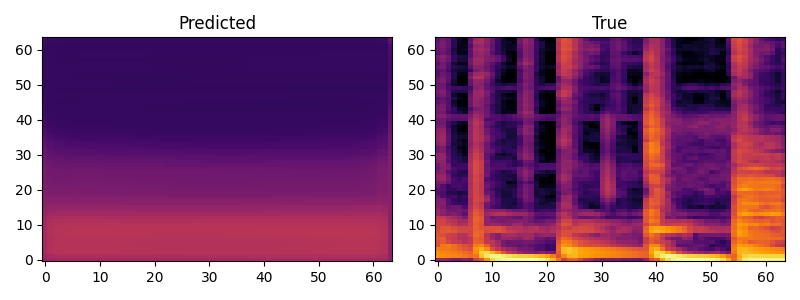
\includegraphics[width=0.48\textwidth]{imgs/spectrograms/media_images_val_spectrograms_8653_82c00f99e0bb079a497f.png} &
    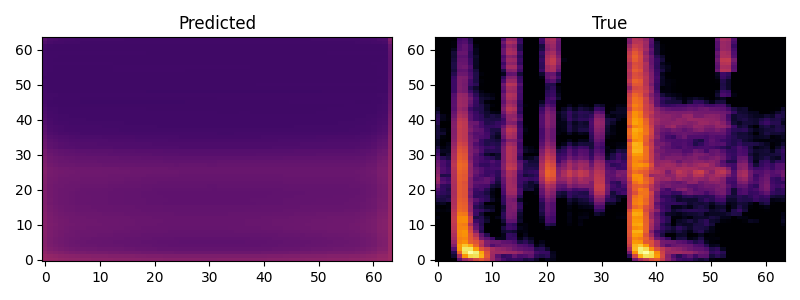
\includegraphics[width=0.48\textwidth]{imgs/spectrograms/media_images_val_spectrograms_8653_8c3ea155cfdde6d1ee92.png} \\
    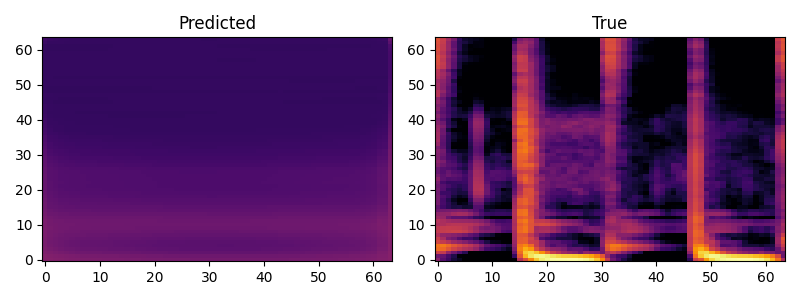
\includegraphics[width=0.48\textwidth]{imgs/spectrograms/media_images_val_spectrograms_8653_8fed809dd87da9f5b5f0.png} &
    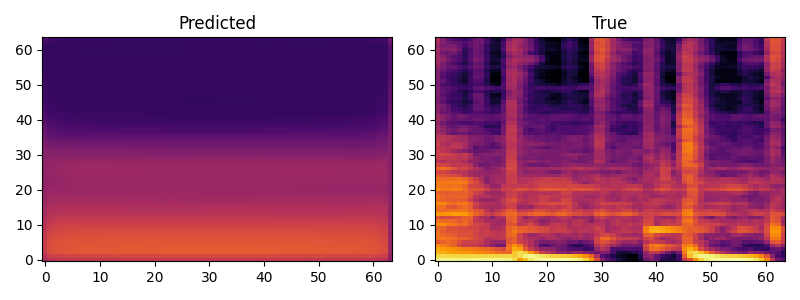
\includegraphics[width=0.48\textwidth]{imgs/spectrograms/media_images_val_spectrograms_8653_f0d90e1a1f7ae3ca67ea.png} \\
    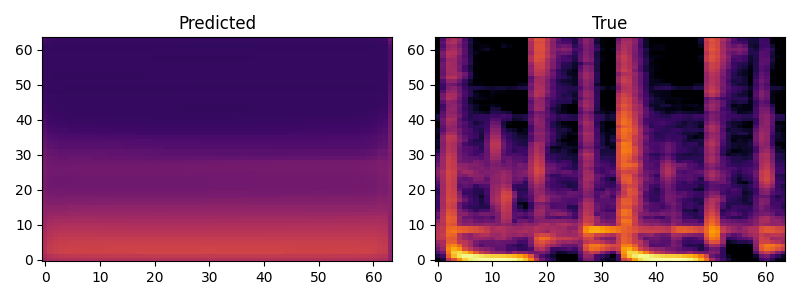
\includegraphics[width=0.48\textwidth]{imgs/spectrograms/media_images_val_spectrograms_8658_54ba5db2984c3817cb8d.png} &
    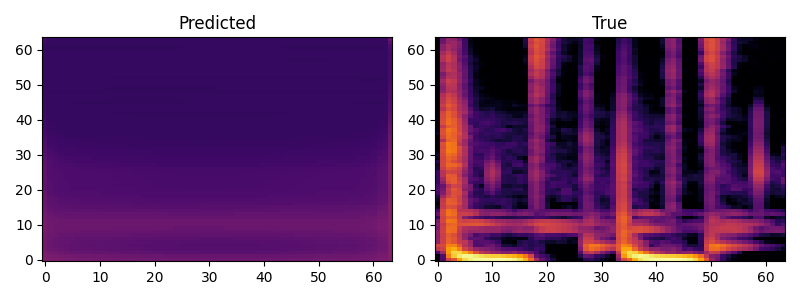
\includegraphics[width=0.48\textwidth]{imgs/spectrograms/media_images_val_spectrograms_8658_7942d7e56630eac823de.png} \\
    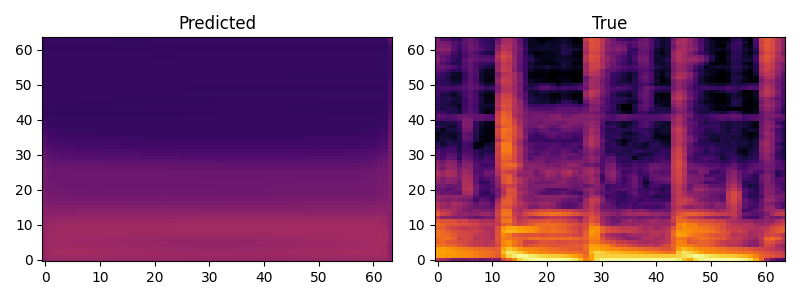
\includegraphics[width=0.48\textwidth]{imgs/spectrograms/media_images_val_spectrograms_8658_7baf70115b8f56210f30.png} &
    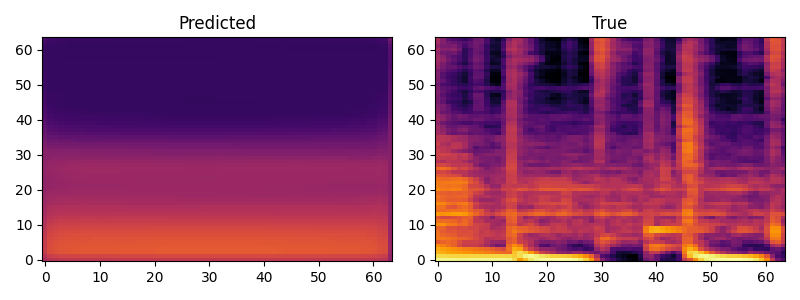
\includegraphics[width=0.48\textwidth]{imgs/spectrograms/media_images_val_spectrograms_8658_9f4076f20a86ba1957bf.png}
  \end{tabular}
  \caption{Reconstructed spectrograms.}
  \label{fig:reconstructed-spectrograms}
\end{figure}

Looking at the reconstructed spectrograms, we can notice that the network has not yet learned the high-resolution temporal aspects of the songs.
It cannot mark note onsets accurately. Instead, it tends to produce smooth spectrograms with almost equally colored rows that show the average power in a frequency band.

\subsection{Time-constant reconstruction}

To test the hypothesis that the network learns to reconstruct an averaged spectrogram for a music fragment, we train a simplified model.
The model has similar architecture to the main CNN model, but instead outputs an image of shape 64x1 which is then broadcasted to the desired shape of 64x64.
With this change we also don't need the full image decoder and therefore keep just a single fully connected layer.

The model is strictly less flexible, but we observe that the results achieved by it are not much worse than the results of the main model.
Comparing these results to the main model we observe few percentage points difference in AUROC scores.

\begin{figure}[h]
  \centering
  \textbf{Accuracy scores for time-constant reconstruction}
  \vspace{0.3cm}
  
  \begin{minipage}[t]{0.48\textwidth}
    \centering
    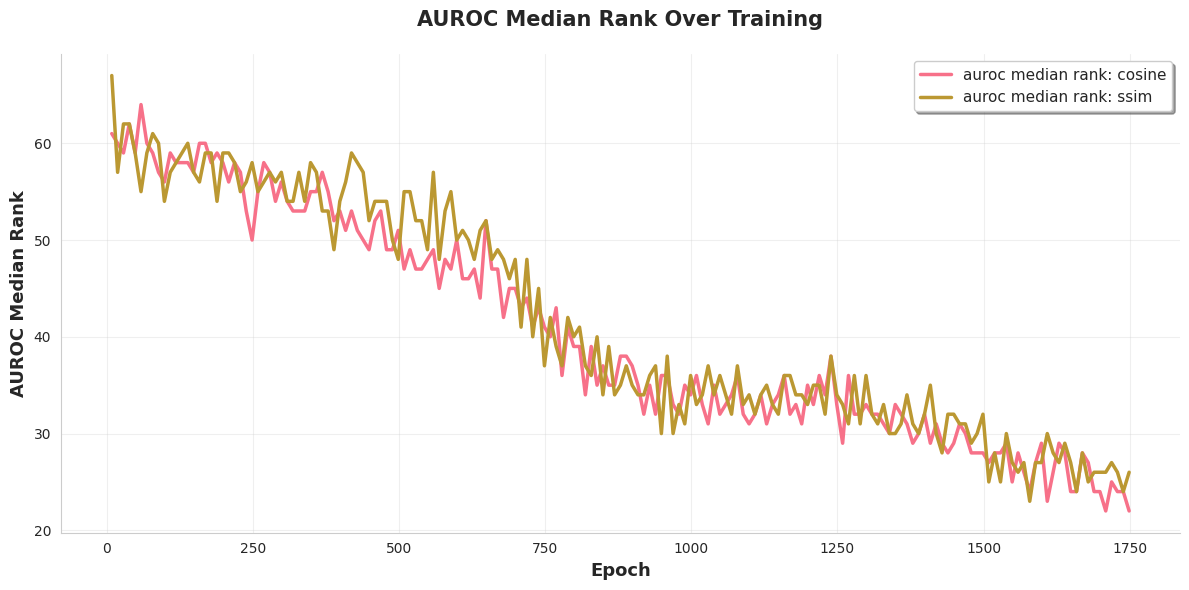
\includegraphics[width=\textwidth]{imgs/medianrank_timeconstant.png}
    \caption{Median rank comparison between the main model and the time-constant model. The time-constant model achieves similar performance despite its reduced flexibility.}
    \label{fig:medianrank-timeconstant}
  \end{minipage}
  \hfill
  \begin{minipage}[t]{0.48\textwidth}
    \centering
    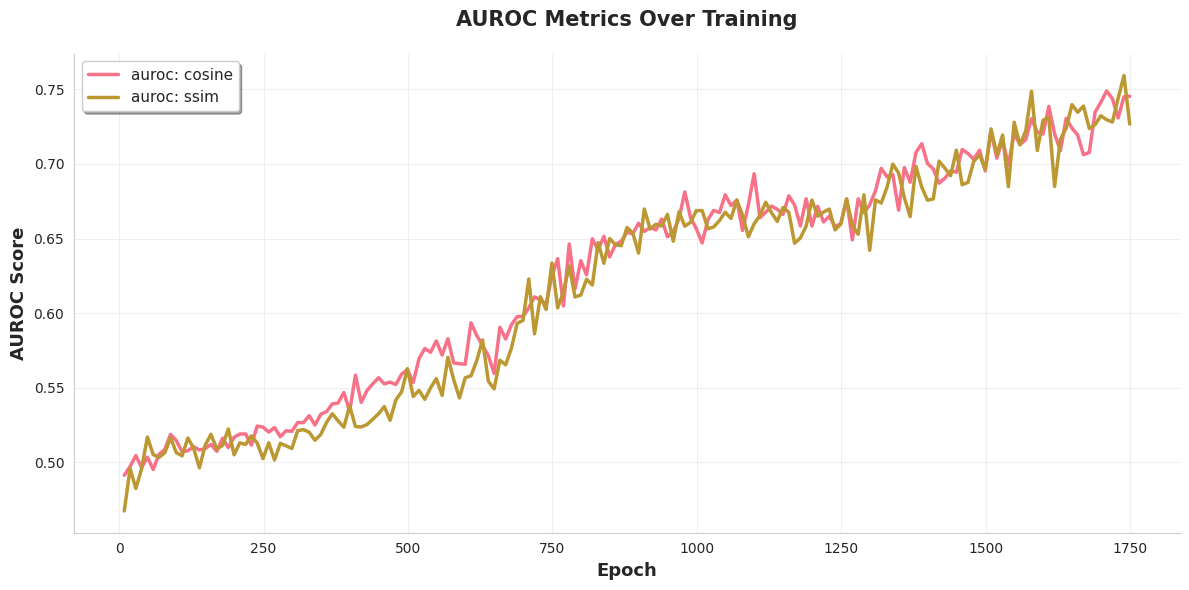
\includegraphics[width=\textwidth]{imgs/auroc_timeconstant.png}
    \caption{AUROC score comparison showing that the time-constant model performs comparably to the full model, supporting the hypothesis that the network learns averaged spectrograms.}
    \label{fig:auroc-timeconstant}
  \end{minipage}
\end{figure}

\begin{figure}[h]
  \centering
  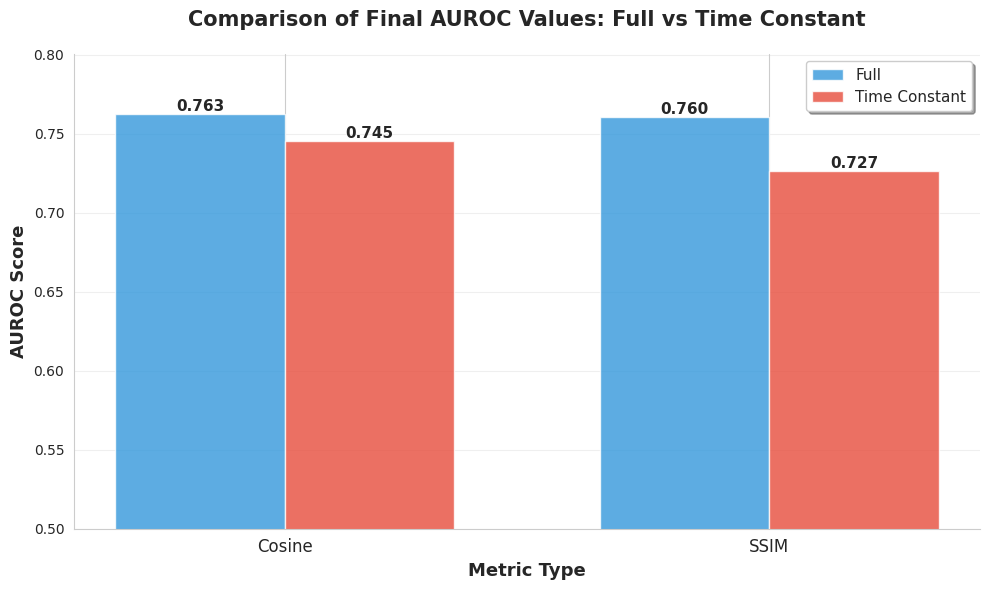
\includegraphics[width=0.7\textwidth]{imgs/auroc_comparison.png}
  \caption{AUROC comparison between the main reconstruction model and the time-constant model.}
  \label{fig:auroc-comparison}
\end{figure}

\section{Attempt at decoding rhytm}

Having decoded the harmonic content we look to rhytm.
The results of full reconstruction suggest that to decode rhytm we need to use different methods.
We take inspiration from \cite{daly} where a Bi-LSTM network is used to perform music decoding in waveform domain.
We aim to predict an onset detection function (ODF), which is a scalar function whose picks indicate sound onsets.
A target ODF is calculated using HFC method which responds to changes in the high frequency part of the spectrogram.
We trained the model on 3 different EEG data types: all 129 EEG channels, only 12 channels hand-picked as relevant to music processing and 12 preprocessed ICA channels.
Separate models are trained for subjects.
We assess quality of predictions by calculating AUROC scores similarly to the mel reconstruction case: we compute similarity to all other ODFs and rank them.

\begin{figure}[h]
  \centering
  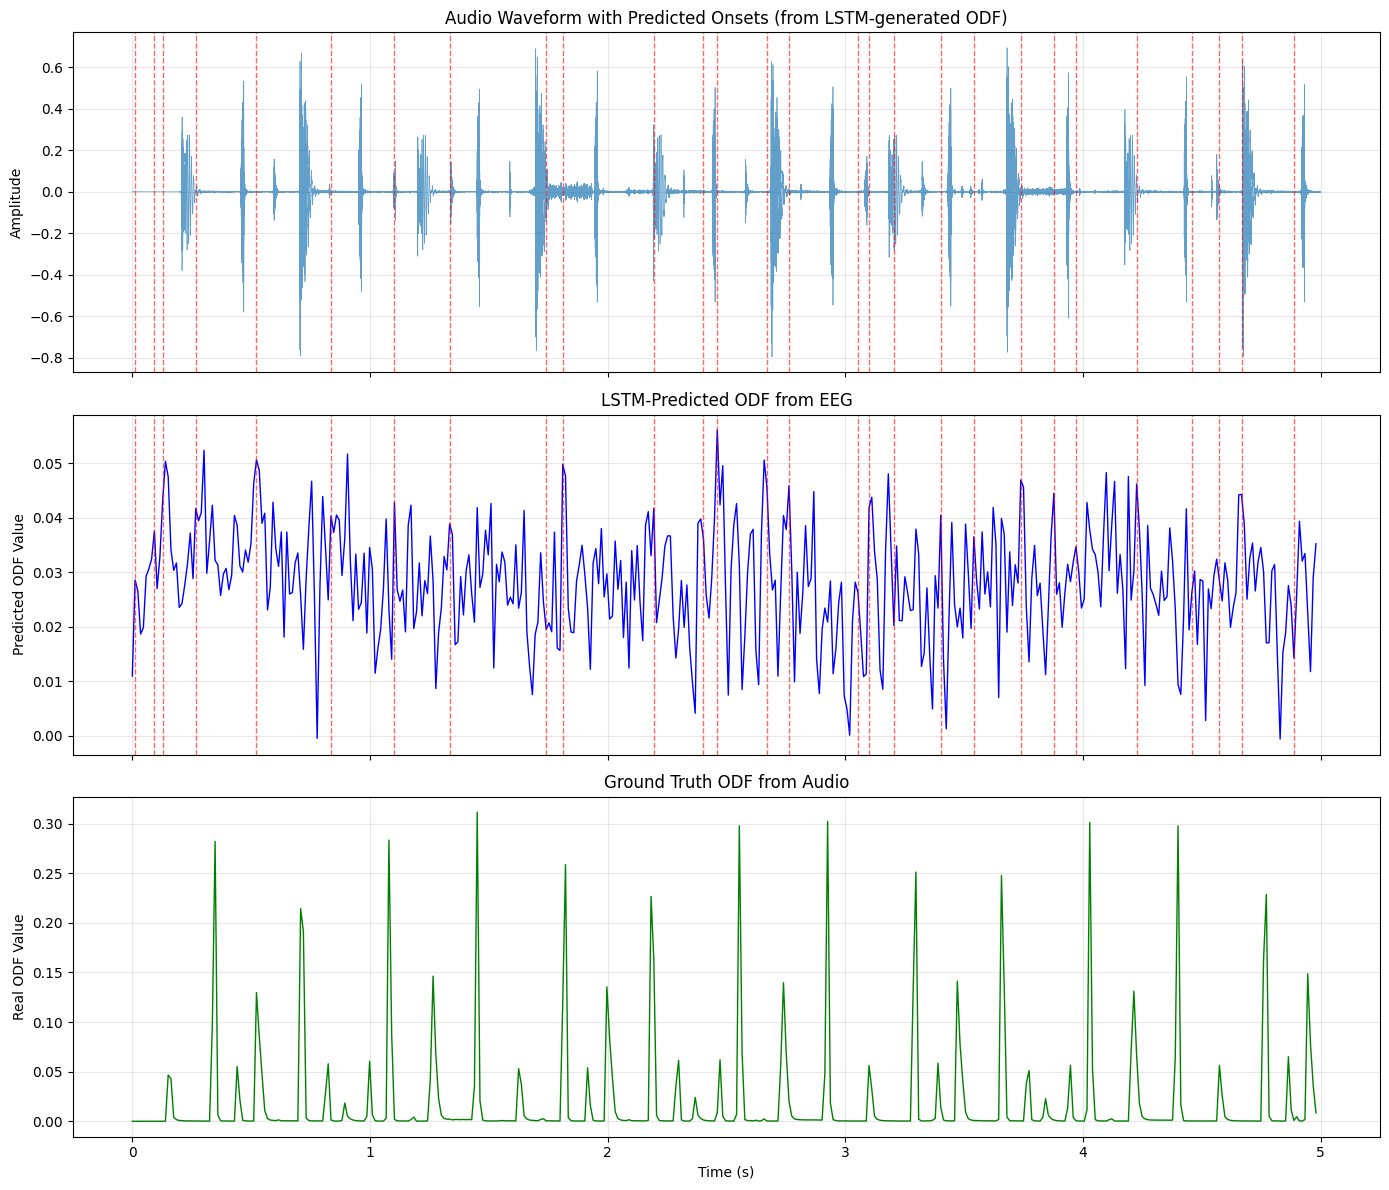
\includegraphics[width=\linewidth]{imgs/lstm_odf_plots.png}
  \caption{LSTM onset detection function plots.}
  \label{fig:lstm-odf-plots}
\end{figure}


In all variants, eventhough we observe training in loss, we do not observe significant results in AUROC scores. Inspecting the predictions visually leaves no doubt in failure of the method.
We also try to overfit the model on single trial, with similar lack of results.

\section{Conclusion and future work}

We had achieved varied success finding features decodable from music to be: song name and music density, but not emotion label. 
We can also reconstruct music in a form of spectrograms.

One could ponder about the use of transformers for below tasks, but we realize that we have unsufficient data to train such models.

% \section{EEG analysis}

% We use this preprocessing with these methods.

% potrzeba: "eeg wygląd", eeg spektrogram, pipeline diagram and pictures, graph acc/subject

% \section{Music id prediction}

% similar:
%  - https://arxiv.org/abs/2009.08793: cnn musin-g
%  - https://www.researchgate.net/publication/360792627_Music_Identification_Using_Brain_Responses_to_Initial_Snippets: 

% \subsection{on musing}

% \subsubsection{12 songs: 90\% }
% \subsubsection{generalization: 20\% }

% \subsection{on bcmi}

% potrzeba: wyniki


\chapter{Discussion}

We have shown the capability of machine learning models to extract music features from EEG data.
We have succeeded in the tasks of song identification, song reconstruction, and a proposed task of music ``density'' prediction.
We have shown applicability of our preprocessing pipeline to machine learning tasks relating music and EEG signals.

Nevertheless, the capability seems limited.
Song identification and reconstruction struggle to generalize across subjects. 
We hypothesize that the datasets are too small for this task, counting only 20 and 10 participants.
Song reconstruction lacks high-resolution temporal details, but the average frequency band power is captured. 
We see this as an extension of the song identification success, where not only a song id but also a specific portion of a song as described by the averaged spectrogram is predicted.
The success of the DTW experiment casts doubt on the claim that the song identification task requires extraction of higher-level features.
We find the optimal performance at the medium model size.
% ____experiment smaller models____
We propose a task of music ``density'' prediction to test the ability for purely musical feature prediction.
We achieve success in that task, but the seemingly mediocre performance of the density prediction model doesn't make the claim fully convincing.
We weren't able to perform rhythm decoding.

The contribution of this work is to demonstrate that machine learning models can extract musically meaningful features from EEG data.
By comparing performance at various tasks using related methods and analyzing the results, we understood better the sources of difficulty in decoding music from EEG.

% \appendix

\chapter{Ablation studies}

\section{Stratified Sampling}

When sampling snippets of specified length from the dataset, we use a stratified sampling approach.
We do this to avoid draws where a snippet is repeatedly sampled from a single region of a trial.
Such an imbalance could lead to overfitting to a portion of the dataset and, generally, to treating various regions disproportionately.
We study the effect of this approach and find that it may matter less than we anticipated.

Recall that the stratified approach means sampling in \( n_{\text{strata}} \) consecutive turns from \( n_{\text{strata}} \) disjoint regions of the sampled dataset.
The parameter \( n_{\text{strata}} \) controls the granularity or the number of disjoint regions summing up to the full trial length.
We perform an experiment where we always sample 100 times from each trial, but vary the number of strata \( n_{\text{strata}} \).
We test on the task of song identification in the MUSIN-G dataset.
The results are shown in the graph below and, at most, seem to suggest a detrimental effect of such sampling when used with the XGBoost model. 
The effect seems small enough that we can follow the intuition behind the stratified approach and use it regardless.

\begin{figure}[H]
  \centering
  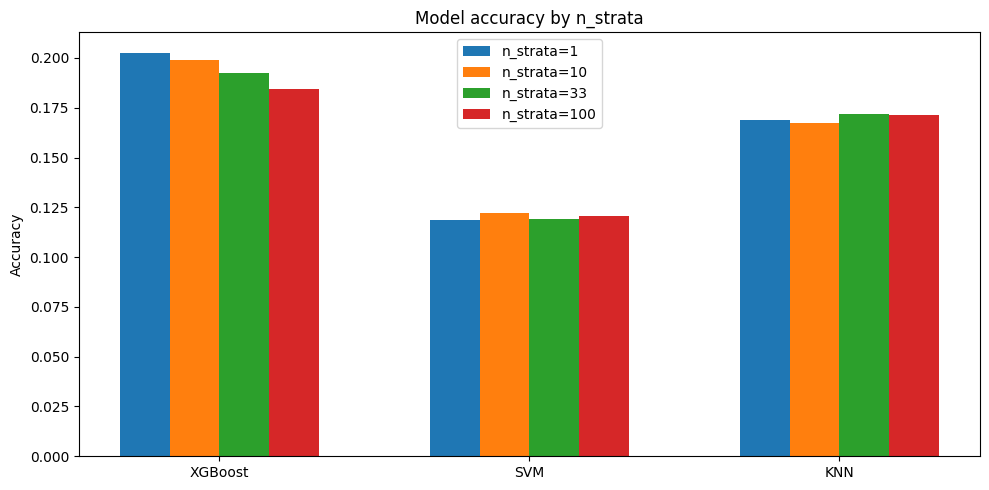
\includegraphics[width=0.8\linewidth]{imgs/stratified_uselesness.png}
  \caption{Effect of stratified sampling on classification accuracy.}
  \label{fig:stratified-sampling-ablation}
\end{figure}


\section{ICA}

In the preprocessing of the EEG data, we use ICA as a dimensionality reduction transform on the EEG signal.
ICA finds a linear transform of the EEG signal into so-called independent components, which are ordered by importance.
Similar to the use of PCA, we can drop the bottom components and reduce the number of channels in the EEG data.
We compare this use of ICA in preprocessing to picking a set of channels and dropping the rest.
The set of channels to be picked in this ``No ICA'' case is predefined and chosen based on proximity to auditory processing regions of the brain or a known relation to music processing.

\begin{figure}[H]
  \centering
  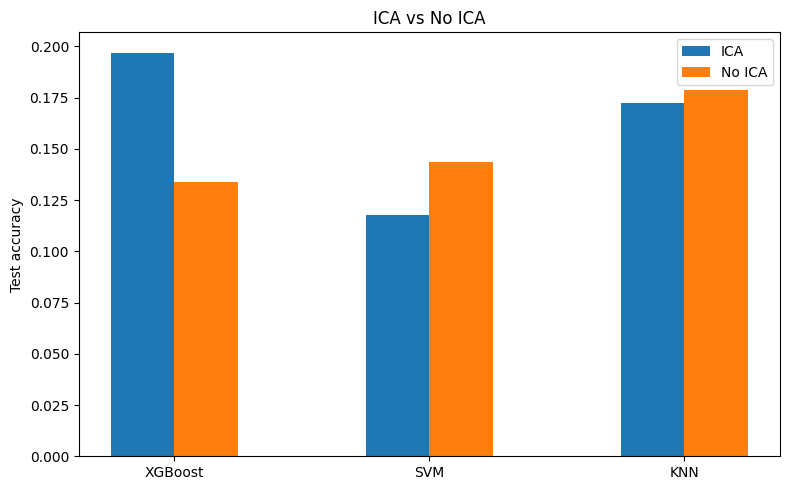
\includegraphics[width=0.8\linewidth]{imgs/ica_usefulness.png}
  \caption{Effect of ICA on classification accuracy.}
  \label{fig:ica-ablation}
\end{figure}

The results as tested on the task of song identification in the MUSIN-G dataset are inconclusive.

\section{Band power features}

For most tasks we employ band power feature analysis to the EEG signal. 
This is almost the last step of our preprocessing pipeline, only before normalization and sampling.
This processing step is crucial, as we are unable to train a model directly on the raw EEG signal.
We attempted song identification---the simplest task---and observed models difficulty to 
not only converge into a meaningful accuracy, but even to minimize the loss function in the first place.
Testing the non-deeplearning methods was omitted due to huge memory use and computation time.

%%%%% BIBLIOGRAFIA

\bibliographystyle{plain}
\bibliography{citations/references,citations/39174725,citations/citations-matteucci1,citations/citations-matteucci3,citations/about_berger,citations/about_vladimir,citations/about_einthoven,citations/about_gibson,citations/rem_sleep,citations/sleep_stage,citations/gloor,citations/fisher,citations/nonstationary,citations/nozaradan,citations/basar,citations/harmony,citations/lal,citations/lagapoulos,citations/klimesch,citations/alastair,citations/engel,citations/ray,citations/bertrand,citations/fries,citations/iclabel,citations/pandey,citations/daly,citations/lawhatre,citations/foster,citations/the-music-of-silence_-part-i_-responses-to-musical-imagery-encode-melodic-expectations-and-acoustics,citations/stober,citations/guess,citations/sterni,citations/rebecca,citations/essentia,citations/sarker,citations/sarker2,citations/musing,citations/bcmi,citations/nicolaou,citations/kello,citations/postolache,citations/controlnet,citations/denk,citations/jain}

\end{document}
